\chapter{Svolgimento dello \textit{stage}} 
\label{cap:descrizione-stage}


\lstset{
   backgroundcolor=\color{lightgray},
   extendedchars=true,
   basicstyle=\footnotesize\ttfamily,
   showstringspaces=false,
   showspaces=false,
   numbers=left,
   numberstyle=\footnotesize,
   numbersep=9pt,
   tabsize=2,
   breaklines=true,
   showtabs=false,
   captionpos=b
}
\section{Flusso di lavoro}
\subsection{Pianificazione delle attività}
In accordo agli obiettivi descritti in \ref{sec:obiettiviStage}, ho redatto, insieme al \textit{tutor} aziendale, una pianficazione settimanale delle attività da svolgere.
Nella tabella \ref{tab:prevAttività} presento la pianificazione di tali attività.

\renewcommand{\arraystretch}{1.5}
\begin{longtable}{|p{3cm}|p{9cm}|} 
    \hline
    \rowcolor{tableheader}\textbf{Periodo} & \textbf{Descrizione attività} \\
    \hline
    \endfirsthead

    \rowcolor{tableheader}\textbf{Periodo} & \textbf{Descrizione attività} \\
    \hline
    \endhead

    \hline
    \endfoot

    \hline
    \endlastfoot
    \rowcolor{tableevenrow} Prima settimana  & \begin{tabular}[t]{@{}p{9cm}@{}}
        - Studio ed apprendimento delle tecnologie di sviluppo \\
        - Definizione delle \textit{user stories} \\
    \end{tabular} \\
    \hline
    \hline
    \rowcolor{tableoddrow} Seconda settimana  &  \begin{tabular}[t]{@{}p{9cm}@{}}
        - Creazione \textit{ticket} di \textit{mock} \\
        - Caricamento dei \textit{ticket} all'interno dell'\gls{its} Jira
    \end{tabular} \\
    \hline
    \rowcolor{tableevenrow} Terza settimana & \begin{tabular}[t]{@{}p{9cm}@{}}
        - Reperire i ticket completati da Jira\\
        - Salvataggio \textit{ticket} su \textit{database} MongoDB \\
        - Aggiornamento costante del \textit{database}\\
    \end{tabular} \\
    \hline
    \rowcolor{tableoddrow} Quarta settimana & \begin{tabular}[t]{@{}p{9cm}@{}}
        - Studio \gls{embedding-g} per \gls{rag-g}\\
        - Tokenizzazione dei \textit{ticket} contenuti nel \textit{database} MongoDB \\
        - Connessione tra AWS Bedrock e MongoDB per \gls{rag-g}\\
    \end{tabular} \\
    \hline
    \rowcolor{tableevenrow} Quinta settimana & \begin{tabular}[t]{@{}p{9cm}@{}}
        - Creazione di domande di \textit{benchmark}\\
        - Confronto tra i diversi \gls{llm}, modelli progettati per generare testo umano\\
    \end{tabular} \\
    \hline
    \rowcolor{tableoddrow} Sesta settimana & \begin{tabular}[t]{@{}p{9cm}@{}}
        - Aggiornamento del \textit{ticket} Jira con la proposta di risoluzione, generata tramite il sistema di IA Generativa\\
        - Sviluppo di un \textit{chatbot} per l'interrogazione sui \textit{ticket} Jira\\
    \end{tabular} \\ 
    \hline
    \rowcolor{tableevenrow} Settima settimana & \begin{tabular}[t]{@{}p{9cm}@{}}
        - Migliorie al sistema di proposte di risoluzione Jira\\
        - Migliorie al \textit{chatbot}, dando all'utente la possibilità di utilizzare \gls{llm} diversi \\
        - Implementare un sistema di autenticazione nel \textit{chatbot} \\
    \end{tabular} \\ 
    \hline
    \rowcolor{tableoddrow} Ottava settimana & \begin{tabular}[t]{@{}p{9cm}@{}}
        - Realizzazione di una presentazione sui progetti sviluppati\\
        - Redazione documento manuale utente \\
        - Redazione documento sull'architettura e sulle scelte progettuali adottate \\
        - Miglioria al \textit{chatbot} per proposte di risoluzione più descrittive \\
    \end{tabular} \\ 
    \hline
    \caption{Pianificazione del progetto di \textit{stage}}
    \label{tab:prevAttività}
\end{longtable}
\noindent
Qui di seguito presento nell'immagine \ref{fig:gantt} che rappresenta la pianificazione delle attività svolte durante il periodo di \textit{stage} tramite un diagramma di Gantt.
\begin{figure}[H]
    \centering
    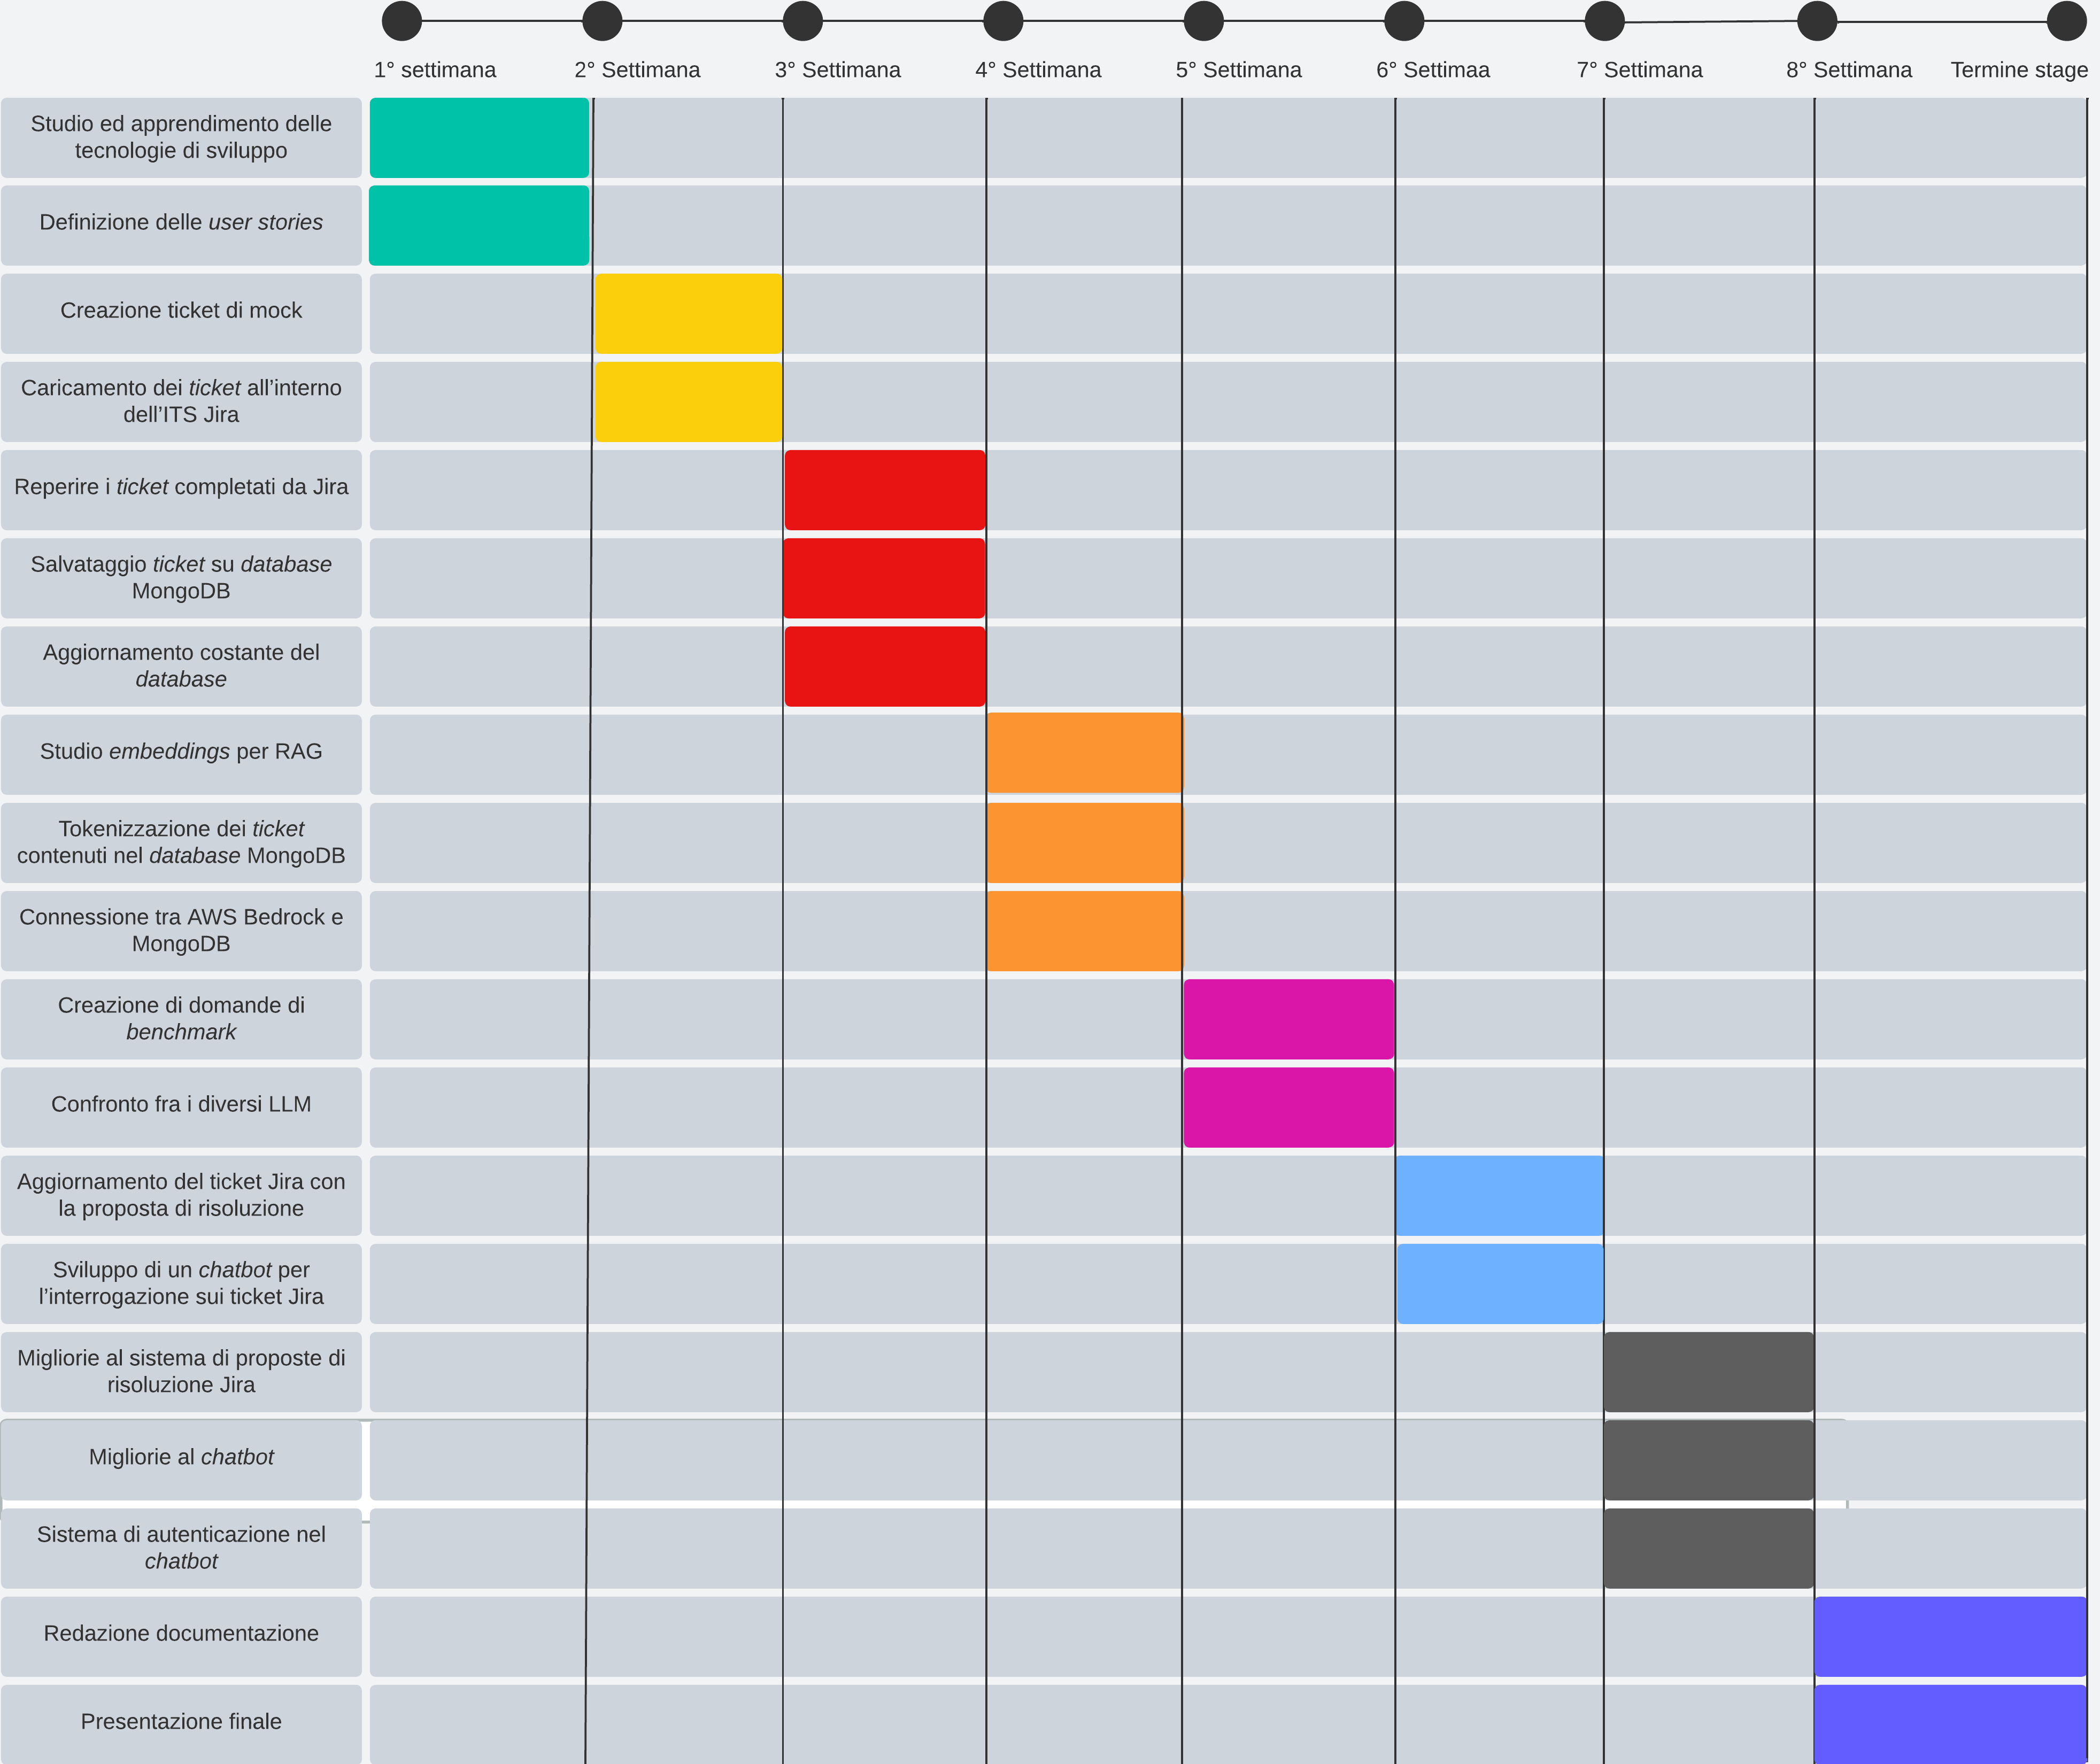
\includegraphics[width=1\textwidth]{diagrammaGantt.png}
    \caption{Diagramma di Gantt delle attività svolte durante lo \textit{stage}}
    \label{fig:gantt}
\end{figure}

\subsection{Revisioni di progetto} \label{sec:revisioni}
L'attività di revisione del progetto ritengo essere stata di fondamentale importanza e più utile ai fini formativi dello \textit{stage}.
Nel corso del tirocinio ho avuto modo di sperimentare due tipologie di revisione: il \textit{daily}, un incontro giornaliero con il \textit{tutor} aziendale, e lo \textit{sprint review}, un incontro settimanale con il \textit{tutor} aziendale per valutare quanto avevo svolto durante la settimana e pianificare le attività per la settimana successiva.
L'occorrenza del \textit{daily} è stata purtroppo però limitata a causa di numerosi impegni che il \textit{tutor} aziendale aveva durante la giornata. Sono stati comunque utili, soprattutto all'inizio dello \textit{stage}, per chiarire dubbi su come procedere con le attività e per ricevere feedback immediato su quanto svolto.
Lo \textit{sprint review} invece è stato quello presente con regolarità assoluta, che mi ha permesso di ricevere un feedback più dettagliato su quanto avevo svolto durante la settimana, che mi hanno permesso di correggere eventuali errori e di migliorare la qualità del lavoro svolto.

\subsection{Interazioni con il tutor aziendale}
Come descritto nella sezione \ref{sec:revisioni}, le interazioni con il \textit{tutor} aziendale sono state numerose e di fondamentale importanza per il corretto svolgimento delle attività.
Nelle giornate in cui non era possibile riferirmi direttamente al \textit{tutor} aziendale, mi sono rivolto ad una figura di supporto, che in caso di assenza o indisponibilità del \textit{tutor} aziendale, era predista all'aiuto degli stagisti in caso di problematiche.


\section{Analisix dei rischi}
I primi giorni di stage sono stati dedicati all'individuazione dei potenziali rischi che avrei potuto incontrare durante lo svolgimento dello \textit{stage}.
Si farà riferimento ai rischi individuati (R) seguendo la seguente notazione: 
\begin{center}
    \textbf{R-[Tipologia]-[Probabilità][Impatto]-[Indice]}
\end{center}
dove:
\begin{itemize}
    \item \textbf{Tipologia}: \\ Natura del rischio: \begin{itemize}
        \item \textbf{T}: Tecnologico
        \item \textbf{O}: Organizzativo
        \item \textbf{P}: Personale
    \end{itemize}
    \item \textbf{Probabilità}: \\ Numero intero positivo che indica la probabilità di occorrenza del rischio: \begin{itemize}
        \item \textbf{1}: Alta
        \item \textbf{2}: Media
        \item \textbf{3}: Bassa
    \end{itemize}
    \item \textbf{Impatto}: \\ Valore alfabetico che indica la probabilità di occorrenza del rischio: \begin{itemize}
        \item \textbf{A}: Alto
        \item \textbf{B}: Medio
        \item \textbf{C}: Basso
    \end{itemize}
    \item \textbf{Indice}: Numero intero positivo incrementale che determina univocamente il rischio relativamente ad una specifica tipologia
\end{itemize}

\renewcommand{\arraystretch}{1.5}
\begin{longtable}{|p{3cm}|p{4.3cm}|p{4.5cm}|} 
    \hline
    \rowcolor{tableheader}\textbf{Codice} & \textbf{Descrizione} & \textbf{Mitigazione} \\
    \hline
    \endfirsthead

    \rowcolor{tableheader}\textbf{Codice} & \textbf{Descrizione} & \textbf{Mitigazione} \\
    \hline
    \endhead

    \hline
    \endfoot

    \hline
    \endlastfoot

    \rowcolor{tableevenrow} R-T-1A-1 & Complessità del contesto di uso di servizi di IA Generativa & 
    Chiedere supporto al \textit{tutor} aziendale sul corretto utilizzo dei servizi di IA Generativa che verranno utilizzati \\
    \hline
    \rowcolor{tableoddrow} R-T-2B-2 & Complessità del contesto di sviluppo e attività di integrazione con la \textit{suite} Atlassian & 
    \begin{tabular}[t]{@{}p{4.3cm}@{}}
        - Riferimento a documentazione più dettagliata \\
        - Supporto da parte del \textit{tutor} aziendale \\
    \end{tabular} \\
    \hline
    \rowcolor{tableevenrow} R-T-1A-3 & Ridotta conoscenza dei servizi cloud \gls{aws} & 
    \begin{tabular}[t]{@{}p{4.3cm}@{}}
        - Studio approfondito dei servizi \gls{aws} \\
        - Documentazione dettagliata dei servizi \gls{aws} \\
        - Supporto da parte del \textit{tutor} aziendale
    \end{tabular} \\
    \hline
    \rowcolor{tableoddrow} R-P-3C-1 & Assenze per motivi di salute o personali & 
    Avvisare per tempo il \textit{tutor} aziendale in caso di ritardi in modo da aggiornare la pianificazione delle attività \\
    \hline
    \rowcolor{tableevenrow} R-O-2A-1 & Lo sviluppo del progetto potrebbe non essere portato a termine nel periodo pianificato a causa di ritardi & 
    Avvisare per tempo il \textit{tutor} aziendale in modo da pianificare le attività per recuperare i giorni di assenza \\
    \hline

    \caption{Analisi dei rischi}
    \label{tab:rischi}
\end{longtable}





\section{Analisi dei requisiti}
\subsection{Aspettative del committente}
In accordo agli obiettivi descritti in \ref{sec:obiettiviStage}, mi è stato richiesto di sviluppare, a seguito di uno studio di fattibilità, un sistema integrato su Jira che alla creazione di un nuovo \textit{ticket}, venisse generata una proposta di risoluzione in base ai \textit{ticket} completati in passato e salvati in un \textit{database} MongoDB.
Inoltre, mi è stato richiesto di sviluppare un \textit{chatbot} che permettesse all'utente di interrogare l'assistente virtuale sui \textit{ticket} Jira e di ricevere proposte di risoluzione.

\subsection{Casi d'uso}
I diagrammi dei casi d'uso permettono di descrivere le interazione tra gli attori e il sistema.  
La convezione che ho utilizzato per la stesura dei casi d'uso è stata la seguente:
\begin{center}
    \textbf{{UC[Numero]}: nome del caso d'uso}
\end{center}
\begin{itemize}
    \item \textbf{UC}: acronimo di \textit{Use Case};
    \item \textbf{Numero}: numero progressivo del caso d'uso. I sottocasi vengono rappresentati nella forma [Numero].[SottoNumero];
\end{itemize}
a cui ho associato una descrizione, la lista degli attori coinvolti, le precondizioni e le postcondizioni affinche il caso d'uso possa avvenire.
Per riassumere i casi d'uso, sono presenti dei diagrammi UML per una rappresentazione grafica degli scenari. Verrano presentati i diagrammi dei casi d'uso principali e non banali dei progetti.
\subsubsection{Attori}
Nel contesto dei casi d'uso, con un attore si definisce chi o cosa interagisce con la specifica funzionalità descritta dal caso d'uso. Ha accesso unicamente alla pagina di \textit{login}; 
Gli attori che ho individuato si suddividono in 2 categorie:
\begin{itemize}
    \item \textbf{Attori principali} \begin{itemize} \item \textbf{Utente generico}: utente che non ha effettuato l'autenticazione nel sistema e del \textit{chatbot}; \item \textbf{Utente amministratore}: utente che ha effettuato l'autenticazione. Ha accesso a tutte le funzionalità del sistema.
    \end{itemize}
    \item \textbf{Attori secondari}: \begin{itemize} \item \textbf{\gls{llm}}: è un attore secondario che permette la generazione di \gls{embedding-g} e di generazione di testo tramite modelli di linguaggio. Questo attore a sua volta può essere interpretato da AmazonTitanV2 (modello di generazione di \gls{embedding-g} offerto da \gls{aws} Bedrock) e da Claude3.5Sonnet (\gls{llm} offerto da \gls{aws} Bedrock).
    \end{itemize}
\end{itemize}
\begin{figure}[H]
    \centering
    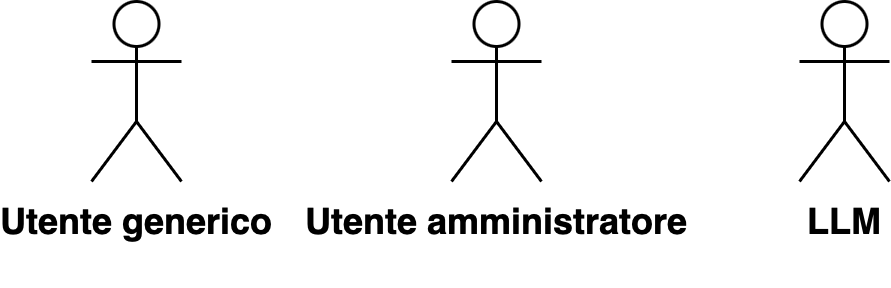
\includegraphics[width=0.55\textwidth]{actors.png}
    \caption{Attori dei casi d'uso}
    \label{fig:attori}
\end{figure}
\subsection*{Lista dei casi d'uso}
\subsubsection{Sistema di proposte di risoluzione Jira}
\subsubsection{UC0: Autenticazione nel \textit{workspace} Jira} 
\textbf{Attori principali}: Utente generico \\
\textbf{Precondizioni}: L'utente vuole accedere al \textit{workspace} Jira \\
\textbf{Descrizione}: All'accesso al \textit{workspace} Jira, viene aperta una schermata di \textit{login} per l'autenticazione dell'utente \\
\textbf{Postcondizioni}: L'utente è autenticato nel \textit{workspace} Jira \\
\begin{figure}[H]
    \centering
    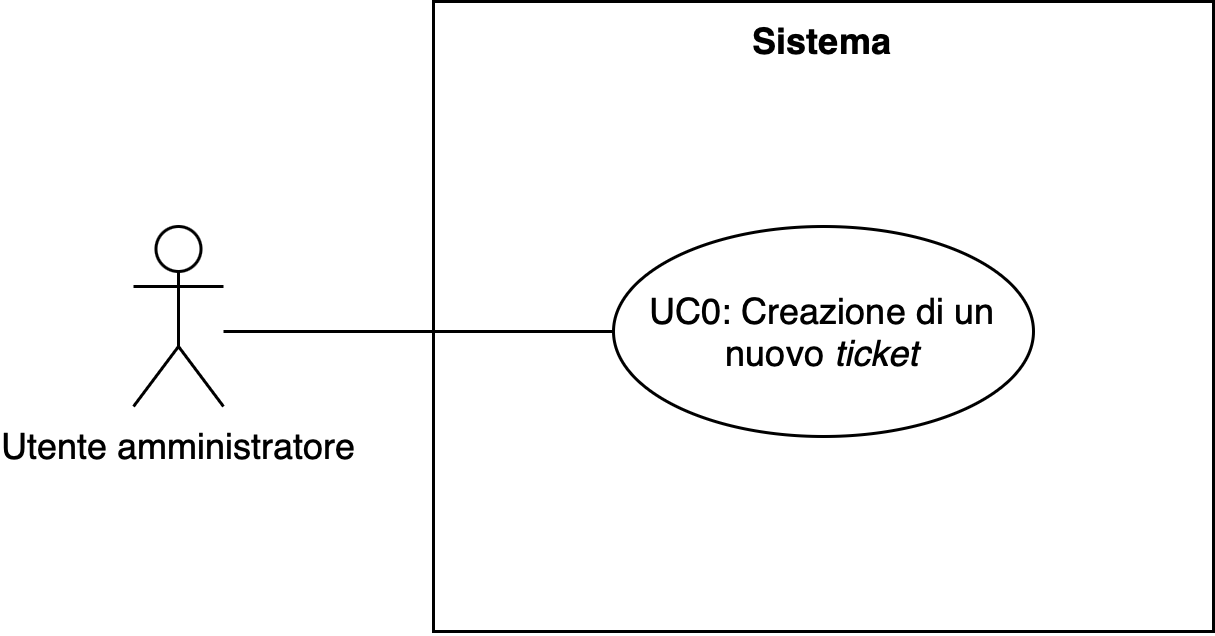
\includegraphics[width=0.55\textwidth]{uc0.png}
    \caption{Diagramma del caso d'uso UC0}
    \label{fig:UC0}
\end{figure}
\subsubsection{UC1: Creazione di un nuovo ticket}
\textbf{Attori principali}: Utente amministratore \\
\textbf{Precondizioni}: L'utente amministratore è autenticato nel \textit{workspace} Jira\\
\textbf{Descrizione}: L'utente amministratore crea un nuovo \textit{ticket} all'interno del progetto Jira \\
\textbf{Postcondizioni}: Il \textit{ticket} è stato creato \\
\begin{figure}[H]
    \centering
    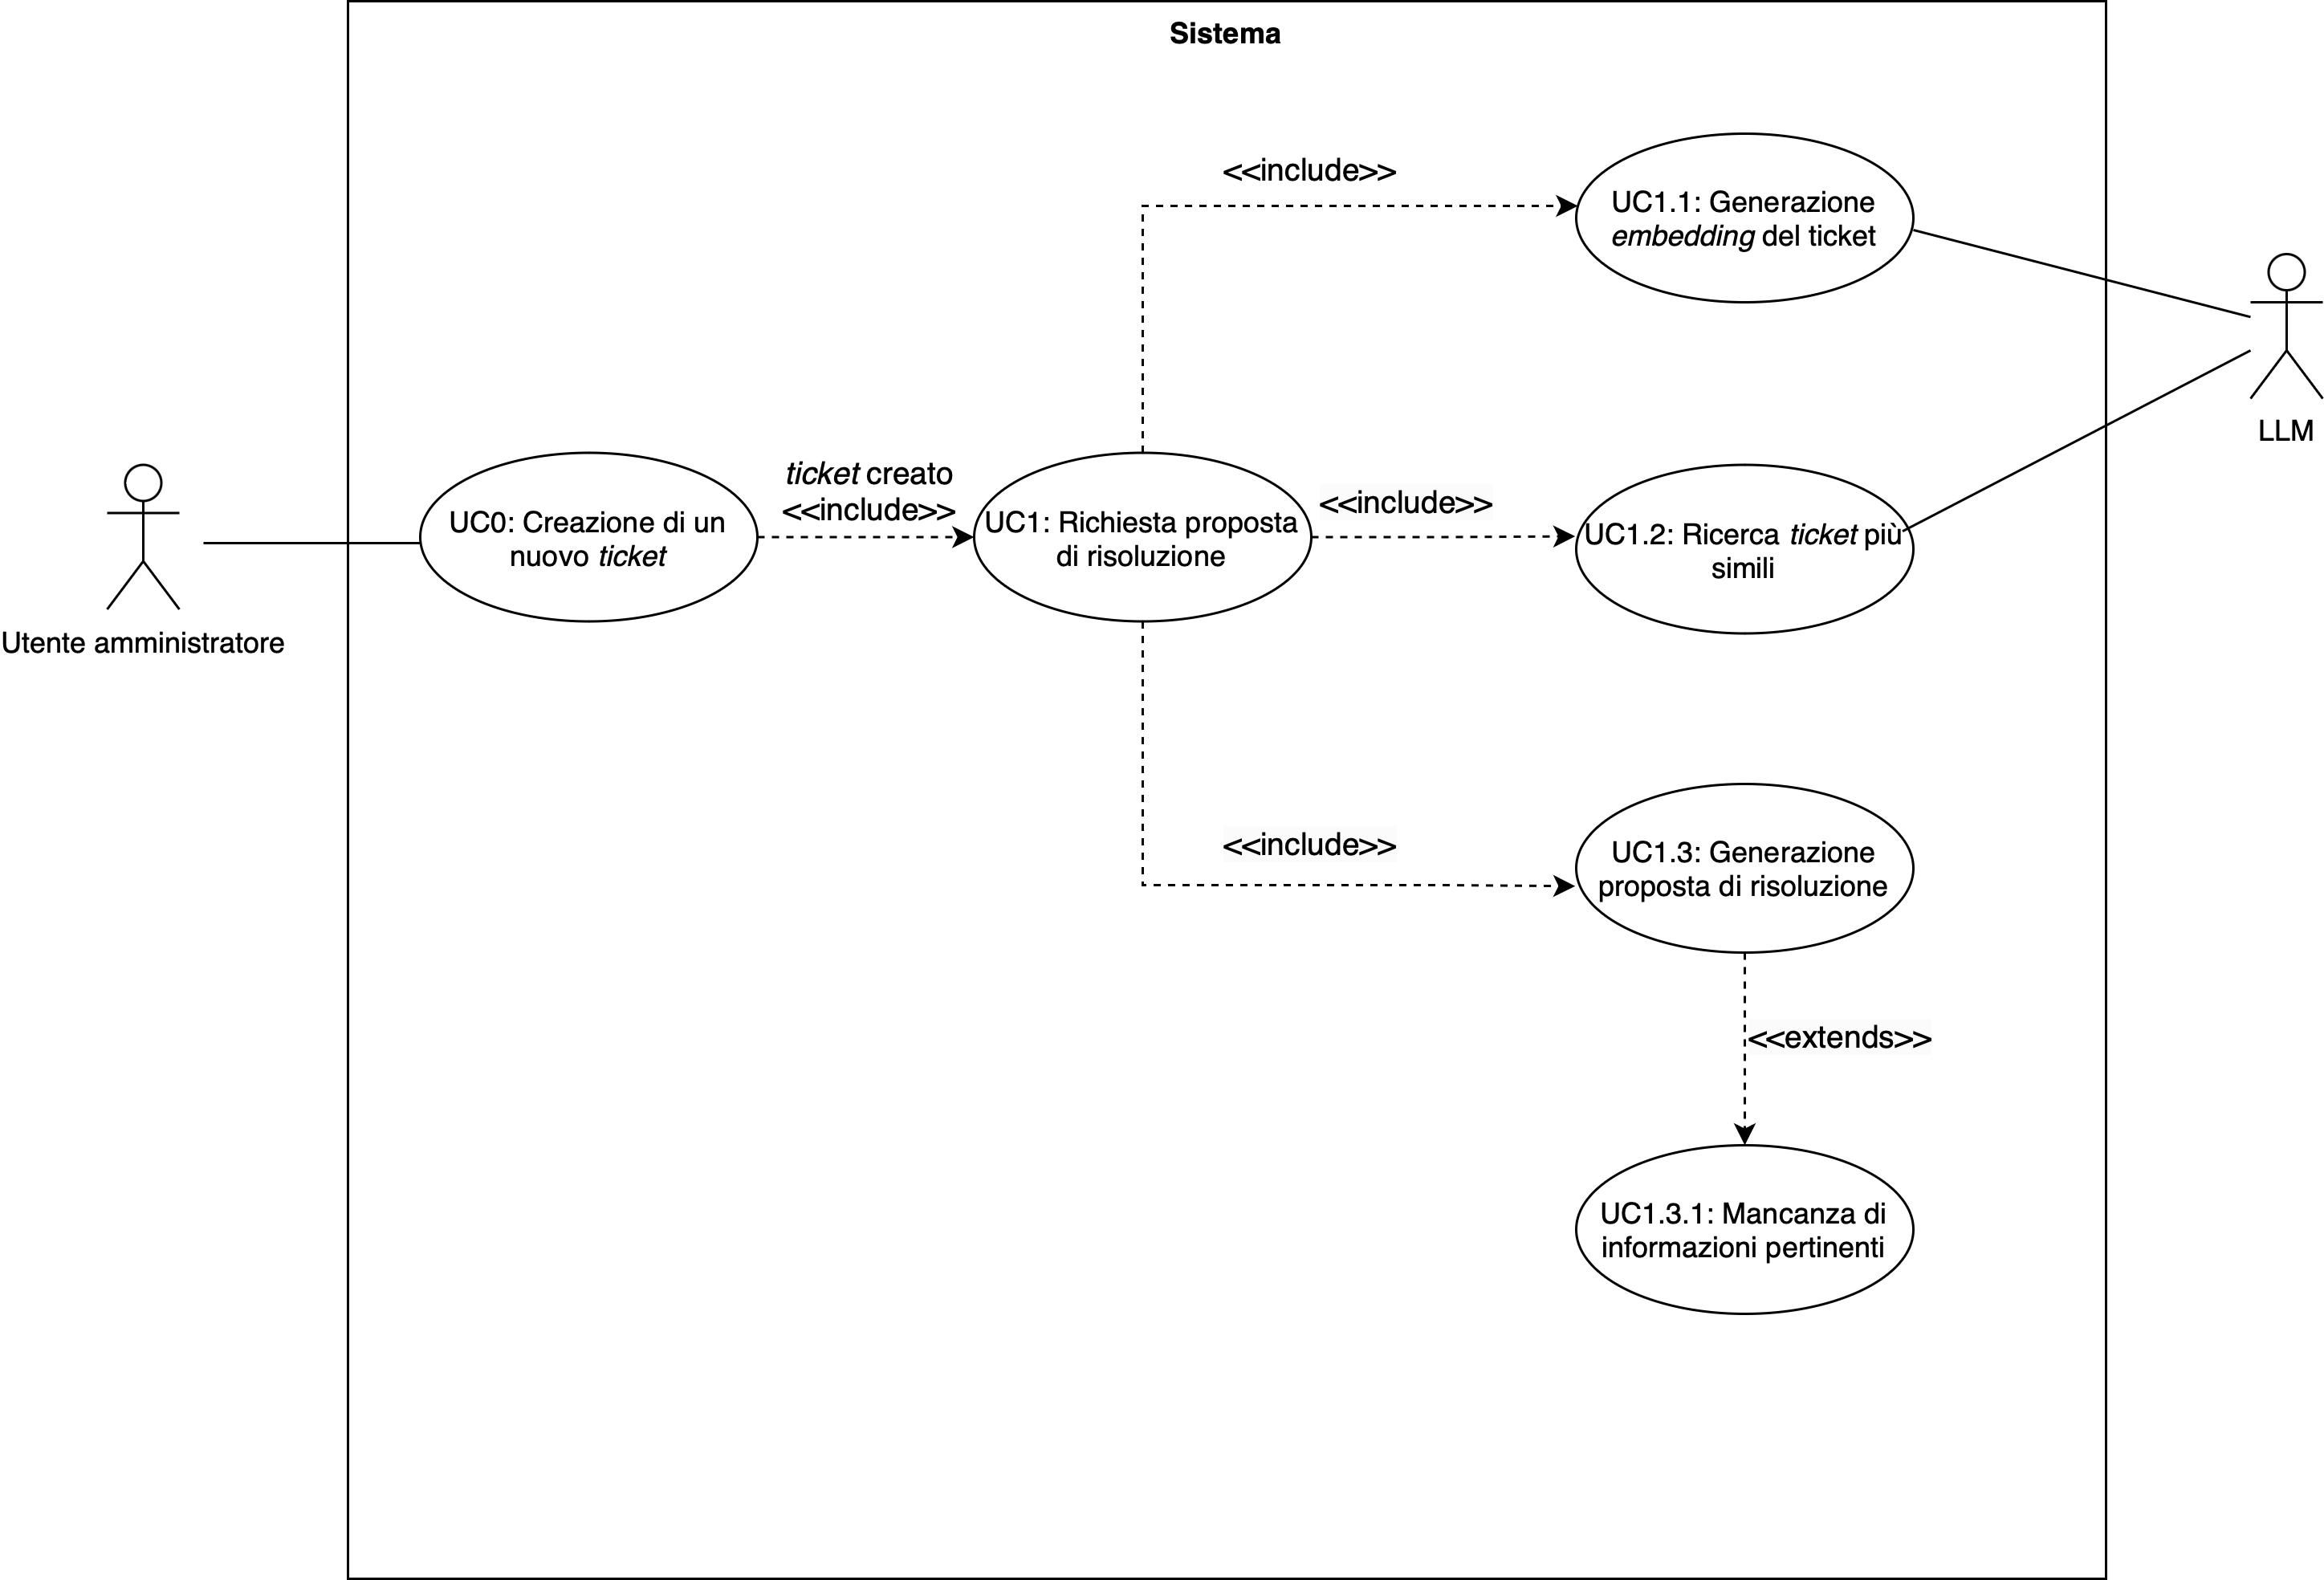
\includegraphics[width=0.55\textwidth]{uc1.png}
    \caption{Diagramma del caso d'uso UC1}
    \label{fig:UC1}
\end{figure}
\subsubsection{UC2: Richiesta proposta di risoluzione}
\textbf{Attori principali}: Utente amministratore \\
\textbf{Precondizioni}: L'utente amministratore ha creato un nuovo \textit{ticket} \\
\textbf{Descrizione}: Viene richiesto al sistema di generare una proposta di risoluzione per il \textit{ticket} appena creato \\
\textbf{Postcondizioni}: Il sistema inizia il processo di generazione della proposta di risoluzione \\

\subsubsection{UC2.1: Generazione \gls{embedding-g} del ticket}
\textbf{Attori principali}: \gls{llm} \\
\textbf{Precondizioni}: Il \textit{ticket} è stato creato ed è stata richiesta una proposta di risoluzione \\
\textbf{Descrizione}: Viene richiesto all'\gls{llm} di generare l'\gls{embedding-g} del \textit{ticket} per effettuare la ricerca dei \textit{ticket} completati più simili \\
\textbf{Postcondizioni}: L'\gls{embedding-g} del \textit{ticket} è stato generato \\

\subsubsection{UC2.2: Ricerca \textit{ticket} più simili}
\textbf{Attori principali}: Sistema \\ 
\textbf{Precondizioni}: È stato generato l'\gls{embedding-g} del \textit{ticket} creato\\
\textbf{Descrizione}: Il sistema effettua una ricerca vettoriale all'interno del \textit{database} con l'utilizzo dell'\gls{embedding-g}, per trovare i \textit{ticket} completati più simili al \textit{ticket} creato \\
\textbf{Postcondizioni}: I \textit{ticket} completati più simili vengono restuiti dal sistema \\

\subsubsection{UC2.3: Generazione proposta di risoluzione}
\textbf{Attori principali}: \gls{llm} \\
\textbf{Precondizioni}: Sono stati restituiti i \textit{ticket} completati più simili al \textit{ticket} creato \\
\textbf{Descrizione}: Viene richiesto all'\gls{llm} di generare una proposta di risoluzione per il \textit{ticket} creato usando come contesto i \textit{ticket} completati più simili \\
\textbf{Postcondizioni}: La proposta di risoluzione è stata generata ed inserita all'interno del campo adibito, del \textit{ticket} creato \\

\subsubsection{UC2.4: Mancanza di informazioni sufficienti}
\textbf{Attori principali}: \gls{llm} \\
\textbf{Precondizioni}: Non sono stati trovati \textit{ticket} completati simili al \textit{ticket} creato \\
\textbf{Descrizione}: Viene generata una risposta standard per informare l'utente amministratore che non sono stati trovati \textit{ticket} completati simili \\
\textbf{Postcondizioni}: Viene inserito un messaggio standard all'interno del campo adibito, del \textit{ticket} creato \\

\begin{figure}[H]
    \centering
    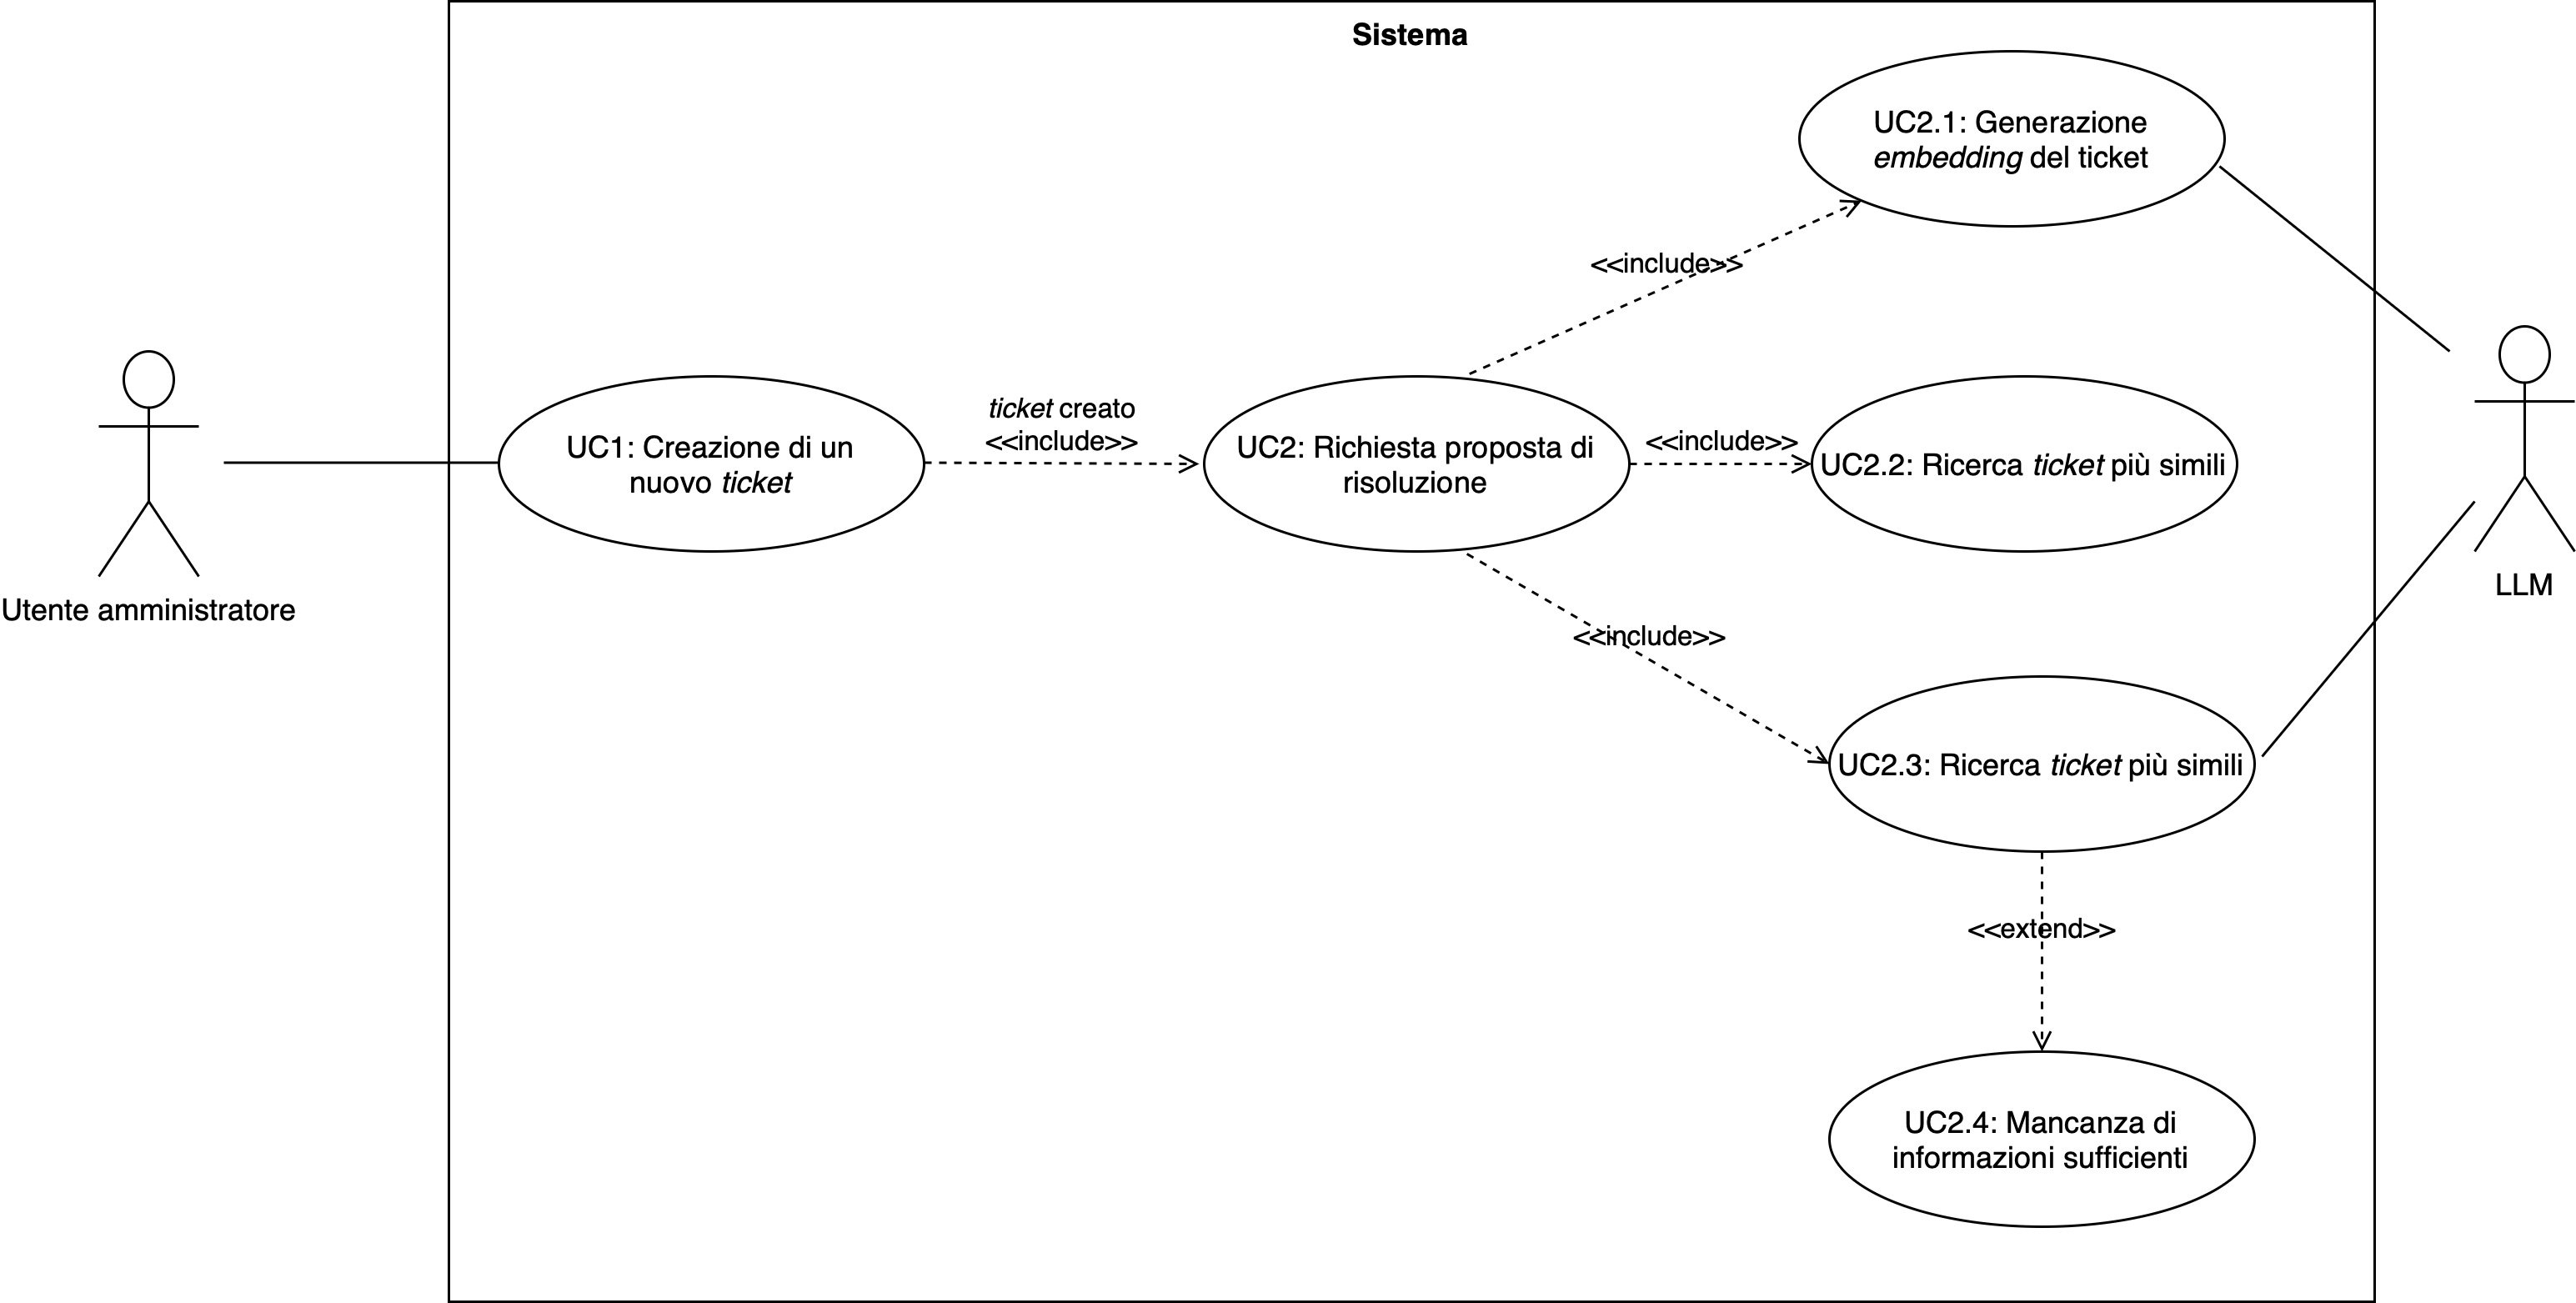
\includegraphics[width=0.95\textwidth]{uc2.png}
    \caption{Diagramma del caso d'uso UC2 e dei relativi sottocasi}
    \label{fig:UC2}
\end{figure}

\subsubsection{UC3: Chiusura di un \textit{ticket}}
\textbf{Attori principali}: Utente amministratore \\
\textbf{Precondizioni}: Il \textit{ticket} è stato completato \\
\textbf{Descrizione}: L'utente amministratore chiude il \textit{ticket} mettondolo in \textit{Done}\\ 
\textbf{Postcondizioni}: Il \textit{ticket} è stato chiuso \\

\begin{figure}[H]
    \centering
    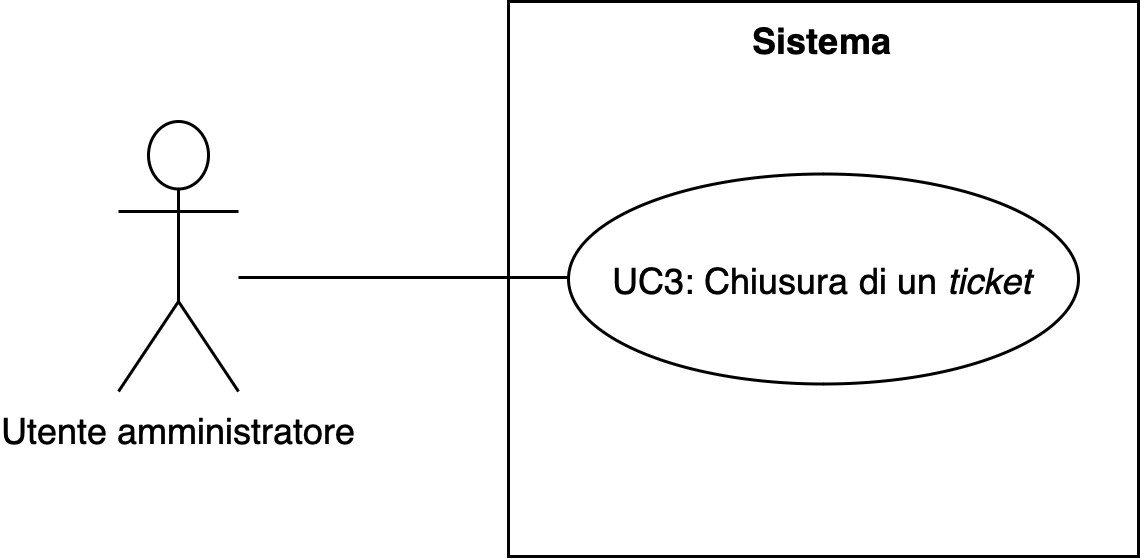
\includegraphics[width=0.55\textwidth]{uc3.png}
    \caption{Diagramma del caso d'uso UC3}
    \label{fig:UC3}
\end{figure}


\subsubsection{UC3.1: Generazione \gls{embedding-g} del \textit{ticket} completato}
\textbf{Attori principali}: \gls{llm} \\
\textbf{Precondizioni}: Il \textit{ticket} è stato chiuso \\
\textbf{Descrizione}: Viene richiesto all'\gls{llm} di generare l'\gls{embedding-g} del \textit{ticket} completato per poterlo poi salvare nel \textit{database} MongoDB \\
\textbf{Postcondizioni}: L'\gls{embedding-g} del \textit{ticket} è stato generato \\

\subsubsection{UC4: Salvataggio \textit{ticket} su \textit{database} MongoDB}
\textbf{Attori principali}: Sistema \\
\textbf{Precondizioni}: Il \textit{ticket} è stato compleato e in stato \textit{Done} \\
\textbf{Descrizione}: Il \textit{ticket} viene salvato su \textit{database} MongoDB con il suo relativo \textit{embedding} \\
\textbf{Postcondizioni}: Il \textit{ticket} è stato salvato su \textit{database} MongoDB con il suo relativo \textit{embedding} \\
\begin{figure}[H]
    \centering
    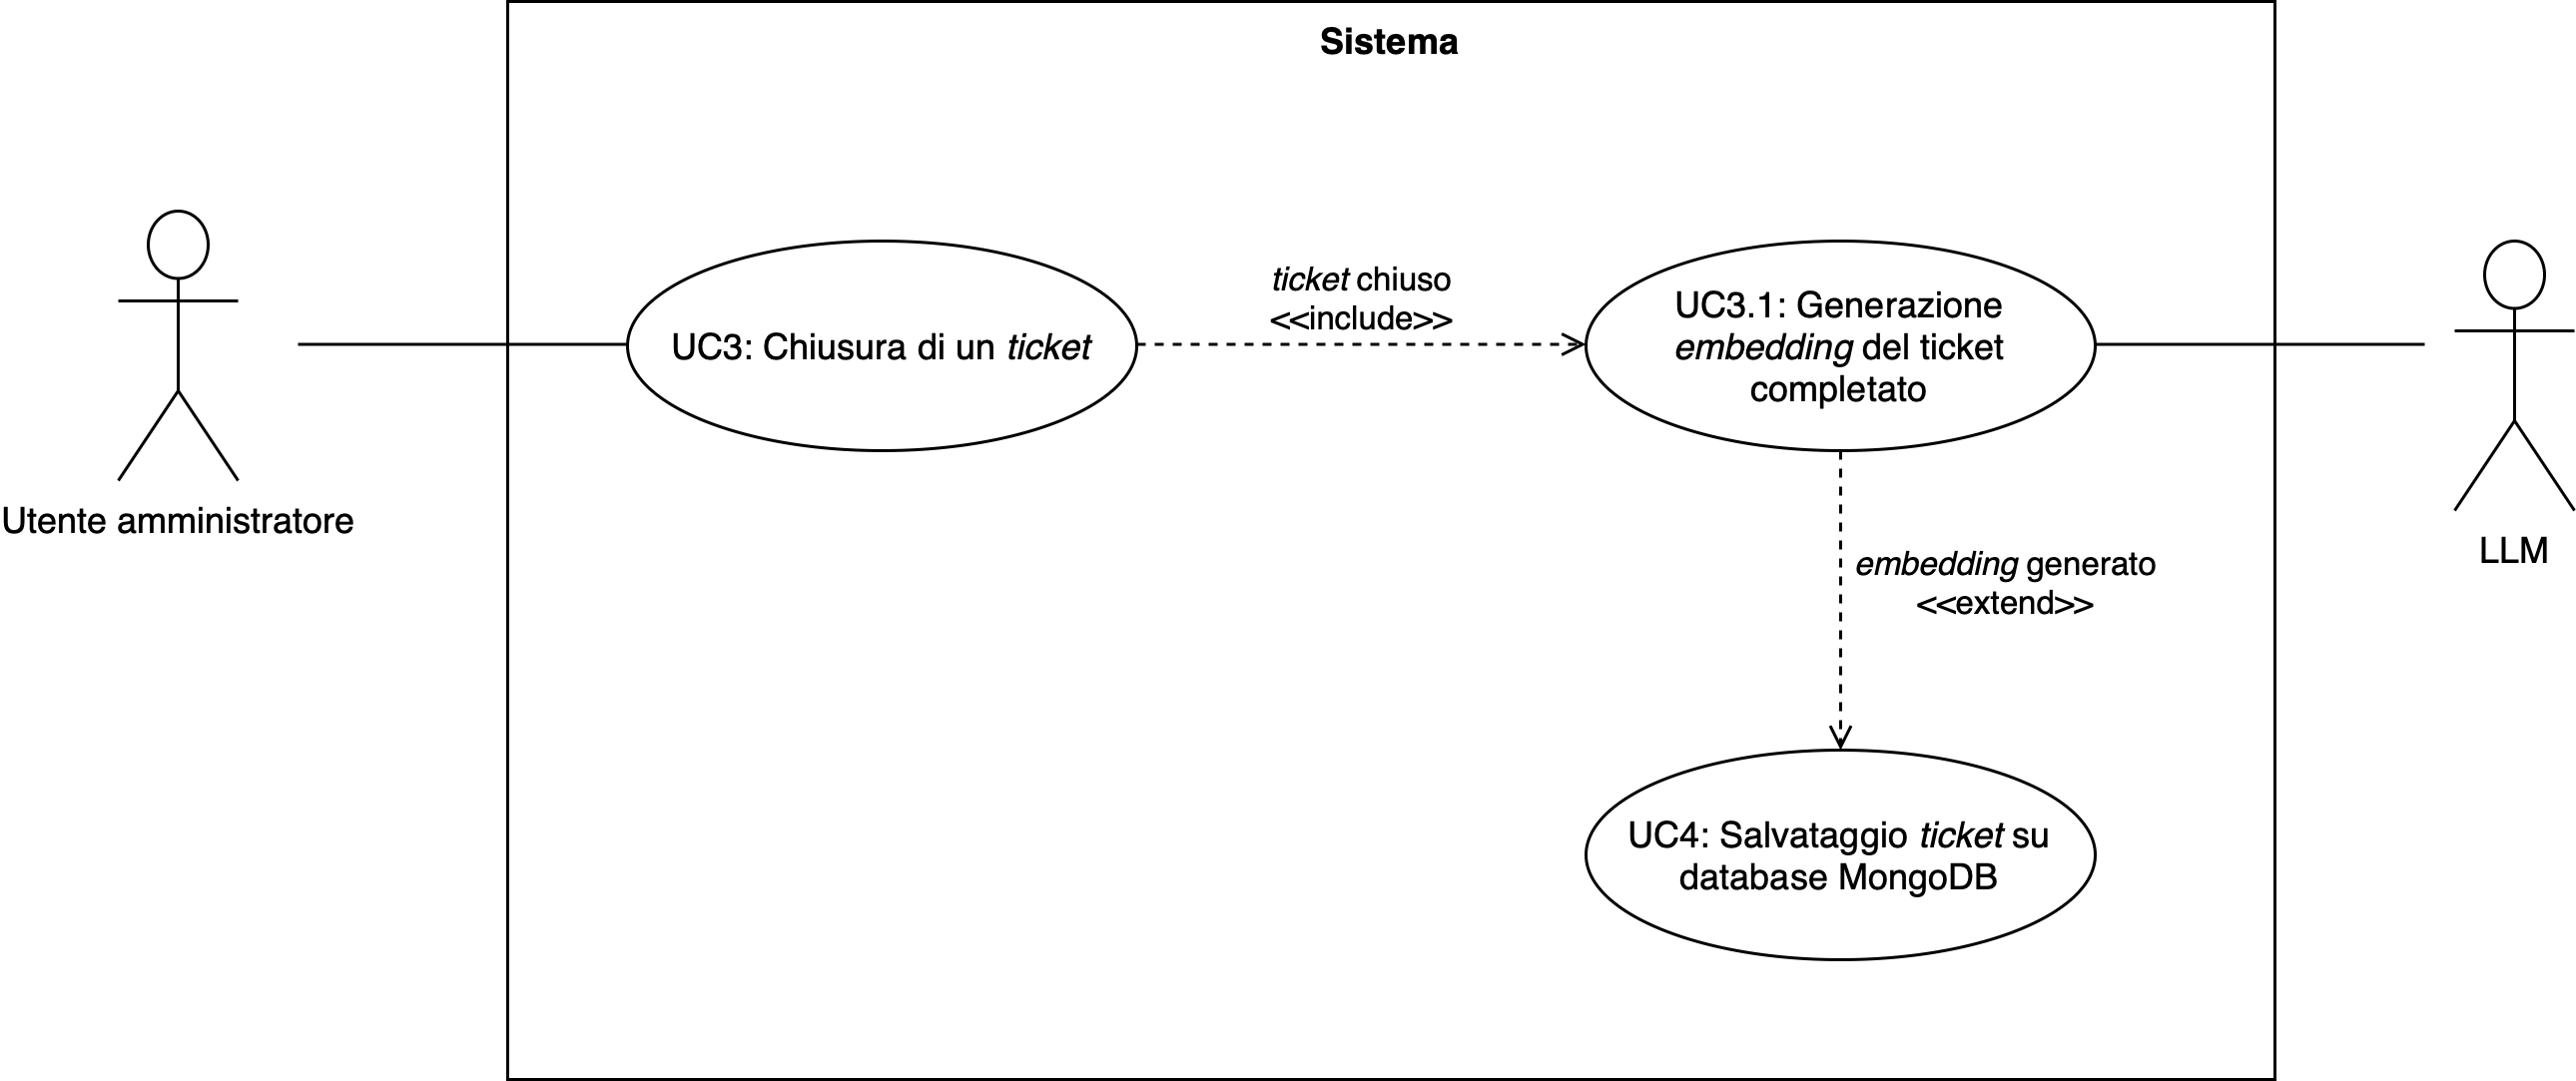
\includegraphics[width=0.75\textwidth]{uc4.png}
    \caption{Diagramma del caso d'uso UC4}
    \label{fig:UC5}
\end{figure}

\subsubsection{\textit{Chatbot}}

\subsubsection{UC0: Autenticazione nel \textit{chatbot}}
\textbf{Attori principali}: Utente generico \\
\textbf{Precondizioni}: L'utente vuole accedere al \textit{chatbot} \\
\textbf{Descrizione}: All'accesso al \textit{chatbot}, viene aperta una schermata di \textit{login} per l'autenticazione dell'utente \\
\textbf{Postcondizioni}: L'utente è autenticato nel \textit{chatbot} \\
\begin{figure}[H]
    \centering
    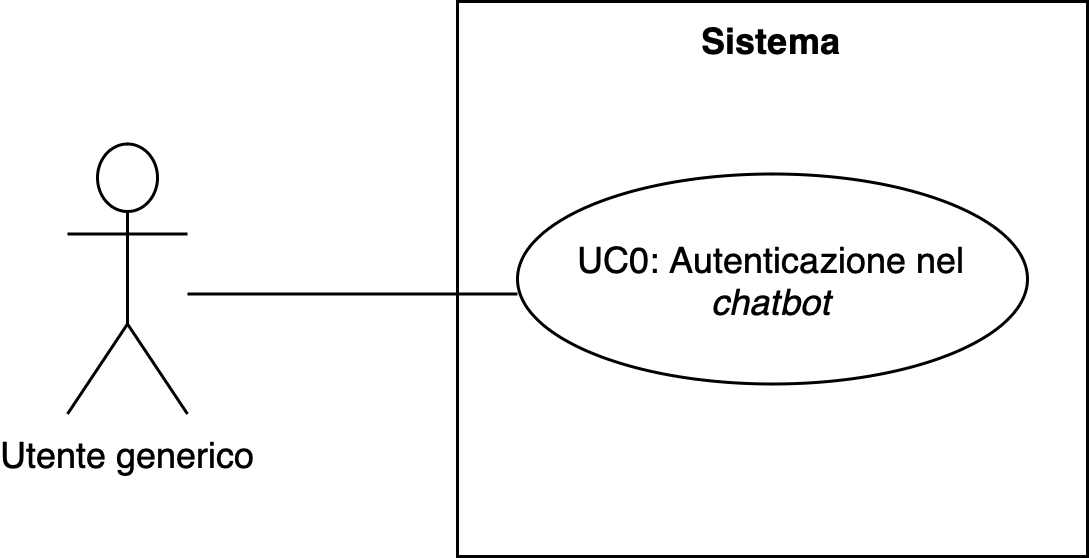
\includegraphics[width=0.55\textwidth]{uc0Chatbot.png}
    \caption{Diagramma del caso d'uso UC0 - \textit{Chatbot}}
    \label{fig:UC0Chatbot}
\end{figure}

\subsubsection{UC1: Autenticazione per il \textit{database} MongoDB}
\textbf{Attori principali}: Utente amministratore \\
\textbf{Precondizioni}: L'utente amministratore è autenticato nel \textit{chatbot} \\
\textbf{Descrizione}: L'utente amministratore si autentica per poter accedere al \textit{database} MongoDB e poter ricercare i \textit{ticket} più simili \\
\textbf{Postcondizioni}: L'utente amministratore è autenticato per il \textit{database} MongoDB \\
\begin{figure}[H]
    \centering
    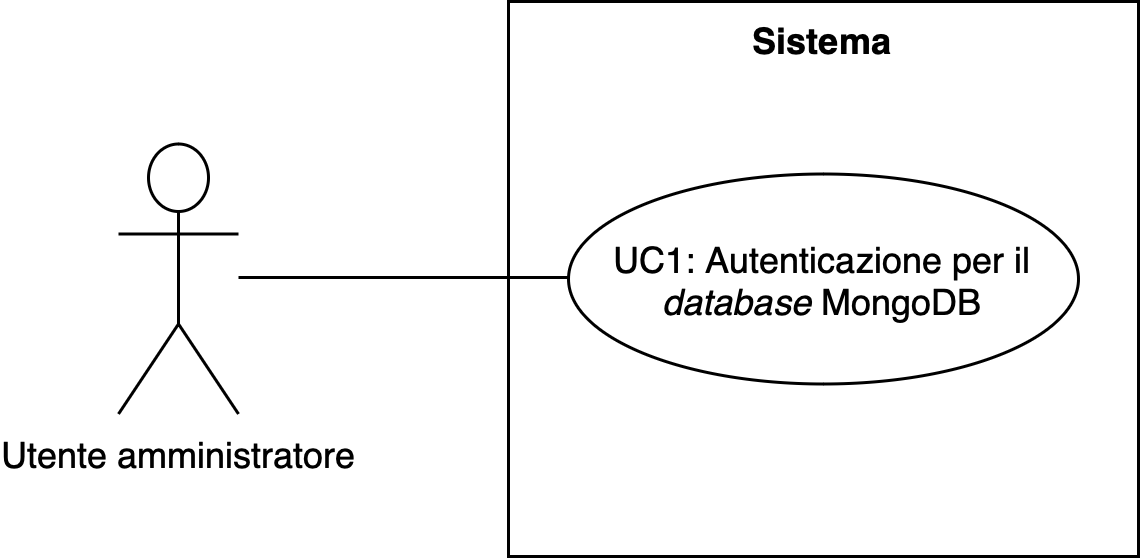
\includegraphics[width=0.55\textwidth]{uc1Chatbot.png}
    \caption{Diagramma del caso d'uso UC1 - \textit{Chatbot}}
    \label{fig:UC1Chatbot}
\end{figure}


\subsubsection{UC2: Scelta del modello \gls{llm}}
\textbf{Attori principali}: Utente amministratore \\
\textbf{Precondizioni}: L'utente amministratore è autenticato nel \textit{chatbot} \\
\textbf{Descrizione}: L'utente amministratore sceglie il modello \gls{llm} con cui interrogare il \textit{chatbot} \\
\textbf{Postcondizioni}: Il modello \gls{llm} è stato scelto \\
\begin{figure}[H]
    \centering
    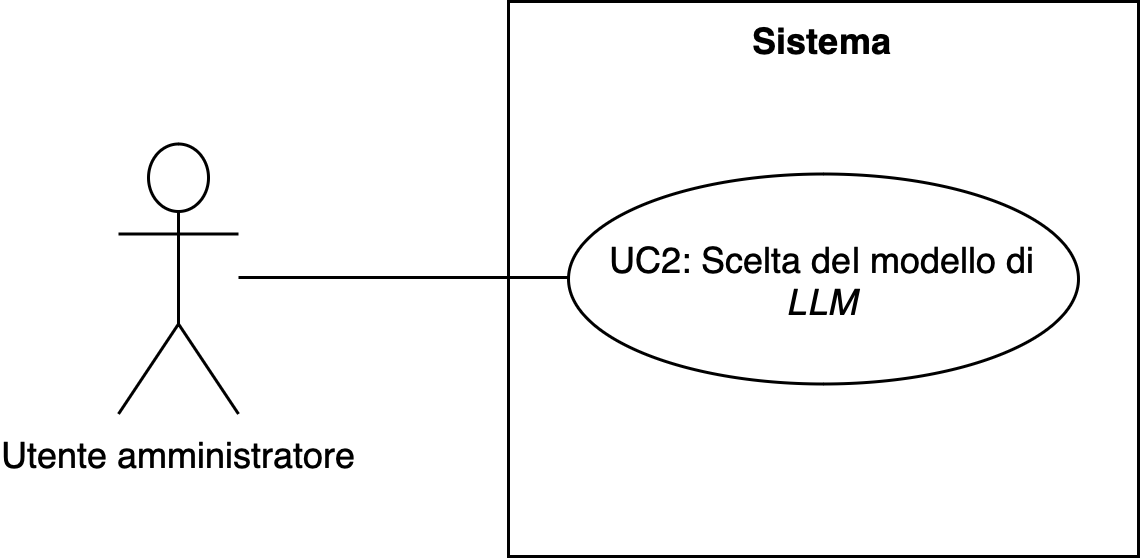
\includegraphics[width=0.55\textwidth]{uc2Chatbot.png}
    \caption{Diagramma del caso d'uso UC2 - \textit{Chatbot}}
    \label{fig:UC2Chatbot}
\end{figure}


\subsubsection{UC3: Inserimento del testo di un \textit{ticket} all'interno della \textit{chat} del \textit{chatbot}}
\textbf{Attori principali}: Utente amministratore \\
\textbf{Precondizioni}: L'utente amministratore ha scelto il modello \gls{llm} con cui interrogare il \textit{chatbot} \\
\textbf{Descrizione}: L'utente amministratore interroga il \textit{chatbot} sui \textit{ticket} Jira \\
\textbf{Postcondizioni}: Il \textit{chatbot} richiede la richiesta di proposta di risoluzione al sistema \\

\subsubsection{UC3.1: Generazione \gls{embedding-g} del testo inserito dall'utente}
\textbf{Attori principali}: \gls{llm} \\
\textbf{Precondizioni}: L'utente amministratore ha inserito il testo del \textit{ticket} per interrogare il \textit{chatbot} \\
\textbf{Descrizione}: Viene generato l'\gls{embedding-g} del testo inserito dall'utente per effettuare la ricerca dei \textit{ticket} completati più simili \\

\subsubsection{U3.2: Ricerca \textit{ticket} più simili all'interno del \textit{database} MongoDB}
\textbf{Attori principali}: Sistema \\
\textbf{Precondizioni}: È stato generato l'\gls{embedding-g} del testo inserito dall'utente \\
\textbf{Descrizione}: Il sistema effettua una ricerca vettoriale all'interno del \textit{database} con l'utilizzo dell'\gls{embedding-g}, per trovare i \textit{ticket} completati più simili al testo inserito dall'utente \\
\textbf{Postcondizioni}: I \textit{ticket} completati più simili vengono restuiti dal sistema \\

\subsubsection{UC3.3: Generazione proposta di risoluzione}
\textbf{Attori principali}: \gls{llm} \\
\textbf{Precondizioni}: Sono stati restituiti i \textit{ticket} completati più simili al testo inserito dall'utente \\
\textbf{Descrizione}: Viene richiesto all'\gls{llm} di generare una proposta di risoluzione per il testo inserito dall'utente usando come contesto i \textit{ticket} completati più simili \\
\textbf{Postcondizioni}: La proposta di risoluzione è stata generata e restituita all'utente, nell'interfaccia del \textit{chatbot} \\


\begin{figure}[H]
    \centering
    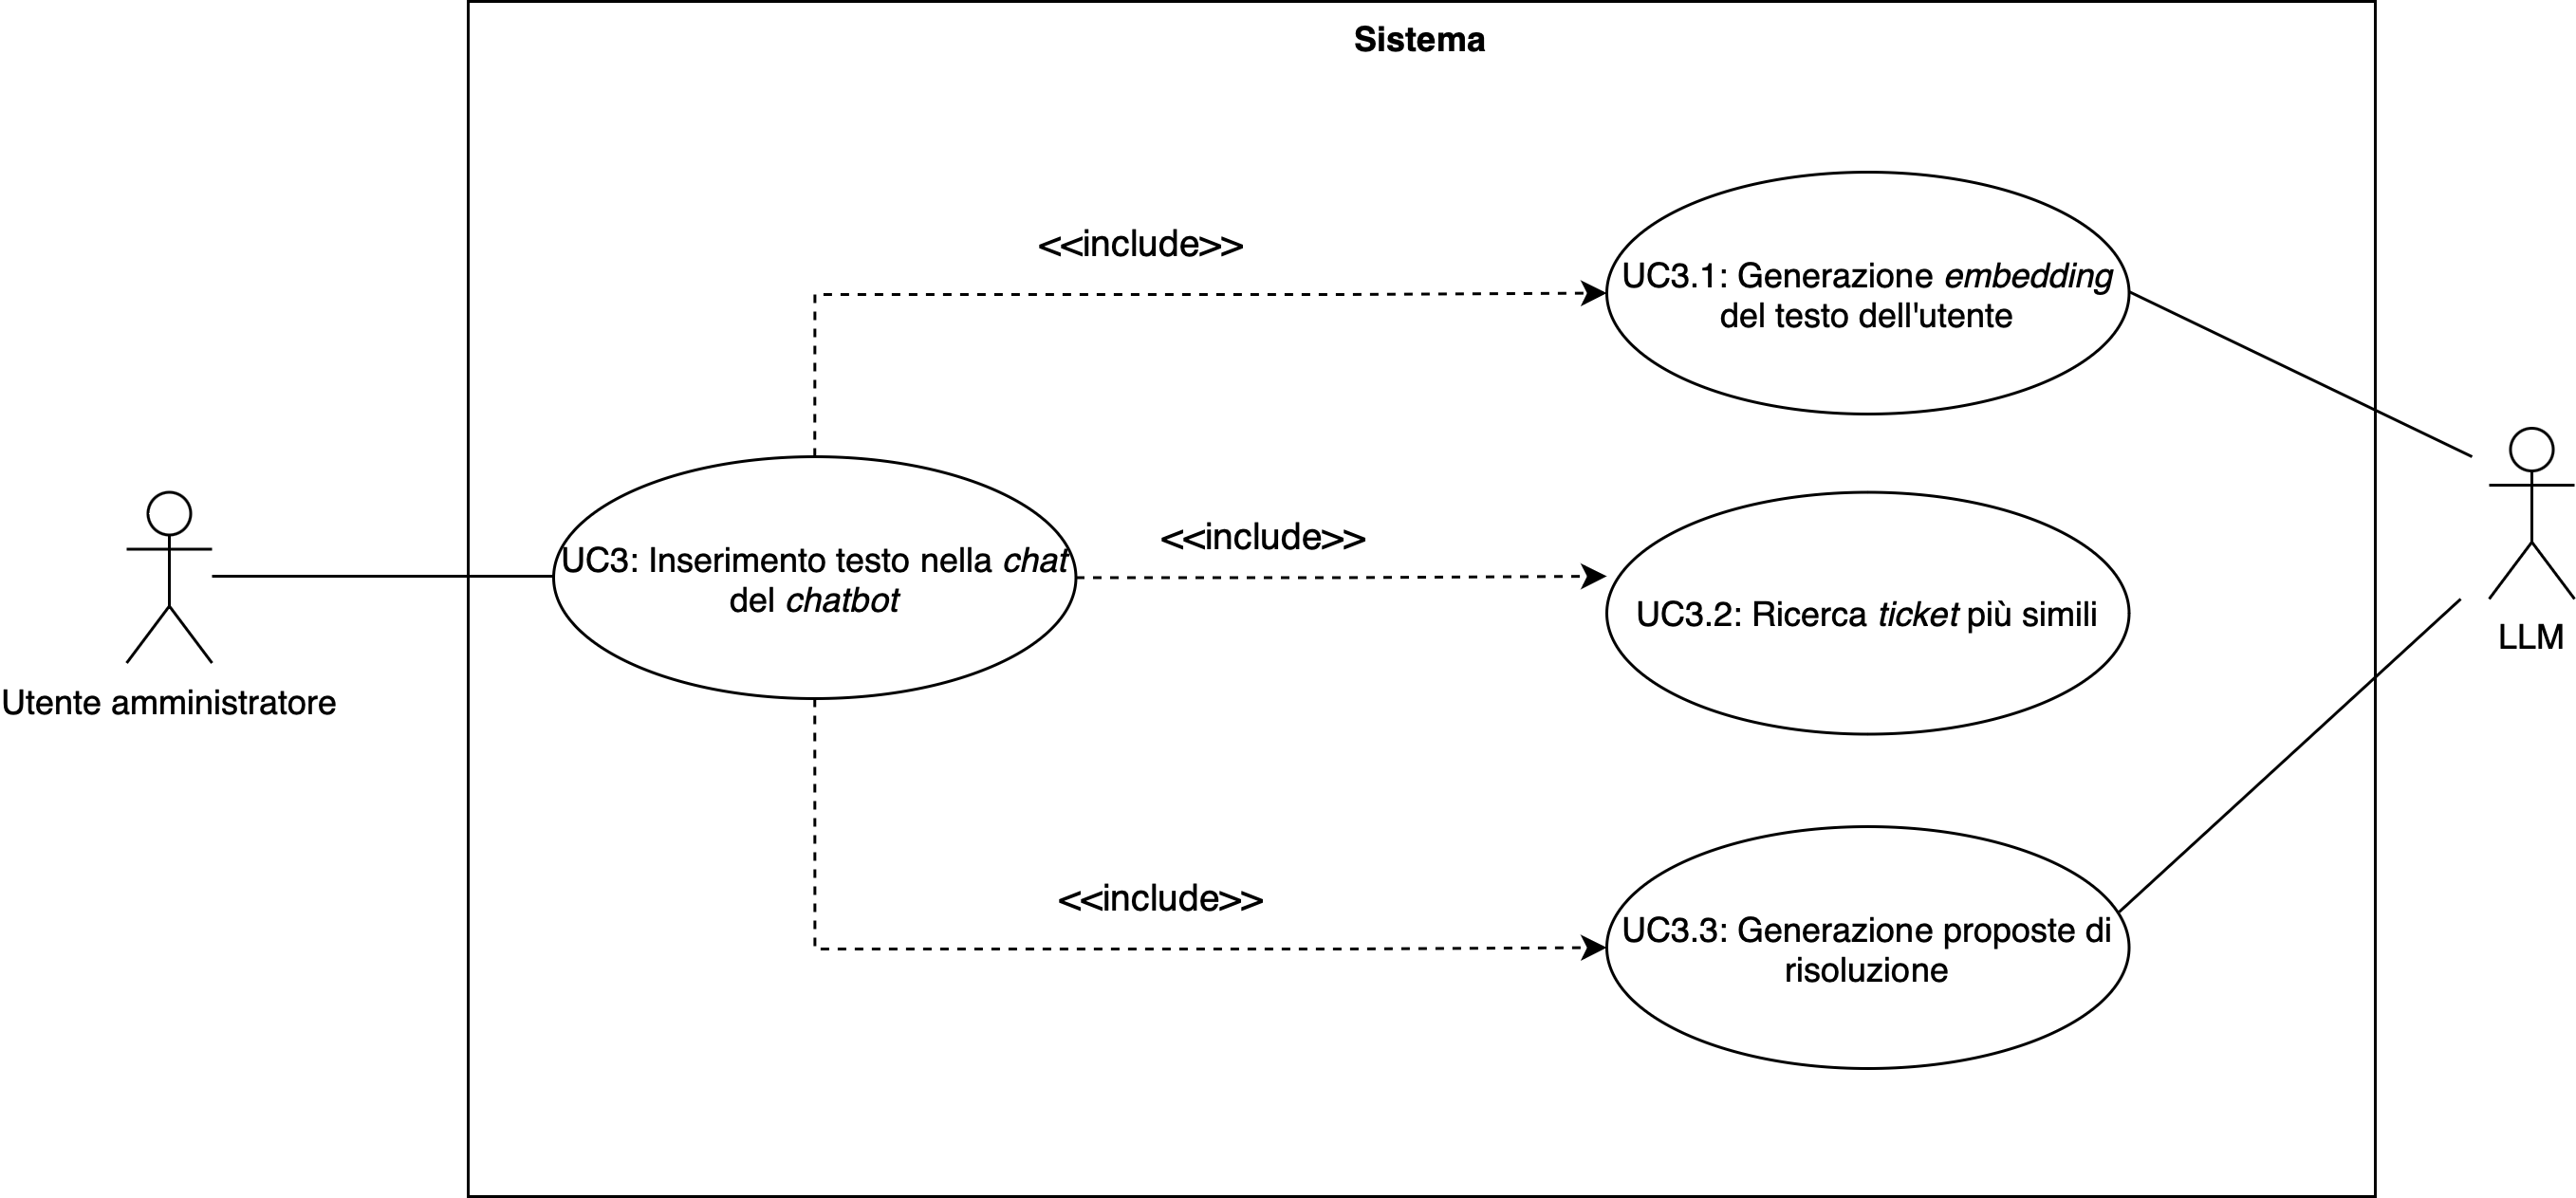
\includegraphics[width=0.95\textwidth]{uc3Chatbot.png}
    \caption{Diagramma del caso d'uso UC3 e dei relativi sottocasi - \textit{Chatbot}}
    \label{fig:UC3Chatbot}
\end{figure}

\subsection{Tracciamento dei requisiti}
Ho tracciato i requisiti individuati dai casi d'uso con la seguente notazione:
\begin{center}
    \textbf{R-[Tipologia][Importanza]-[Numero]}
\end{center}
dove: 
\begin{itemize}
    \item \textbf{Tipologia}: Natura del requisito: \begin{itemize}
        \item \textbf{F}: Funzionale
        \item \textbf{V}: Vincolo
    \end{itemize}
    \item \textbf{Importanza}: Valore alfabetico che indica l'importanza del requisito: \begin{itemize}
        \item \textbf{O}: Obbligatorio
        \item \textbf{D}: Desiderabile
        \item \textbf{O}: Opzionale
    \end{itemize}
    \item \textbf{Numero}: Numero intero positivo progressivo del requisito
\end{itemize}

\renewcommand{\arraystretch}{1.7}
\begin{longtable}{|p{1.5cm}|p{5.5cm}|p{2cm}|p{2.5cm}|} 
    \hline
    \rowcolor{tableheader}\textbf{Codice} & \textbf{Descrizione} & \textbf{Importanza} & \textbf{Fonte}\\
    \hline
    \endfirsthead

    \rowcolor{tableheader}\textbf{Codice} & \textbf{Descrizione} & \textbf{Importanza} & \textbf{Fonte} \\
    \hline
    \endhead

    \hline
    \endfoot

    \hline
    \endlastfoot
    \hline
    R-FO-1 & Il sistema deve eseguire una richiesta di generazione di proposta di risoluzione quando un \textit{ticket} viene creato & Obbligatorio & UC2 (Jira) \\
    \hline
    R-FO-2 & Il sistema deve poter interrogare un \gls{llm} per la creazione dell'\gls{embedding-g} del \textit{ticket} creato & Obbligatorio & UC2.1 (Jira) \\
    \hline
    R-FO-3 & Il sistema deve effettuare una ricerca dei ticket completati più simili al \textit{ticket} creato, nel \textit{database} & Obbligatorio & UC2.2 (Jira) \\
    \hline
    R-FO-4 & Il sistema deve poter interrogare un \gls{llm} per generare una proposta di risoluzione utilizzando come contesto i \textit{ticket} completati più simili. & Obbligatorio & UC2.3 (Jira) \\
    \hline
    R-FO-5 & Il sistema deve poter interrogare un \gls{llm} per generare una risposta standard in caso di mancanza di \textit{ticket} completati simili. & Obbligatorio & UC2.4 (Jira) \\
    \hline
    R-FO-6 & Il sistema deve poter interrogare un \gls{llm} per la generazione dell'\gls{embedding-g} del \textit{ticket} completato per salvarlo nel \textit{database} & Obbligatorio & UC3.1 (Jira) \\
    \hline
    R-FO-7 & Il sistema deve permettere il salvataggio del \textit{ticket} completato e del relativo \gls{embedding-g} nel \textit{database}. & Obbligatorio & UC4 (Jira) \\
    \hline
    R-FO-8 & Il sistema deve permettere l'autenticazione dell'utente nel \textit{chatbot}. & Obbligatorio & UC0 (Chatbot) \\
    \hline
    R-FO-9 & Il sistema deve permettere l'autenticazione dell'utente amministratore per accedere al \textit{database}. & Obbligatorio & UC1 (Chatbot) \\
    \hline
    R-FO-10 & Il sistema deve permettere la scelta del modello \gls{llm} con cui interrogare il \textit{chatbot}. & Obbligatorio & UC2 (Chatbot) \\
    \hline
    R-FO-11 & Il sistema deve permettere l'interrogazione al modello \gls{llm-g} tramite una \textit{chat}. & Obbligatorio & UC3 (Chatbot) \\
    \hline
    R-FO-12 & Il sistema deve poter interrogare un \gls{llm} per generare l'\gls{embedding-g} del testo inserito dall'utente. & Obbligatorio & UC3.1 (Chatbot) \\
    \hline
    R-FO-13 & Il sistema deve permettere la ricerca dei ticket più simili all'interno del \textit{database}. & Obbligatorio & UC3.2 (Chatbot) \\
    \hline
    R-FO-14 & Il sistema deve poter interrogare un \gls{llm} per la generazione di una proposta di risoluzione basata sui \textit{ticket} simili. & Obbligatorio & UC3.3 (Chatbot) \\
    \hline
    R-VO-15 & Il sistema Jira deve essere sviluppato utilizzando il Serverless \textit{framework}  & Obbligatorio & Interna \\
    \hline
    R-VO-16 & Il \textit{database} utilizzato deve essere MongoDB & Obbligatorio & Interna \\
    \hline
    R-VO-17 & Il \textit{chatbot} deve essere sviluppato utilizzando il \textit{framework} Streamlit & Obbligatorio & Interna \\
    \hline
    R-VO-18 & L'autenticazione nel \textit{chatbot} deve utilizzare il servizio \gls{aws} Cognito & Obbligatorio & Interna \\

    
    \hline
    \caption{Pianificazione del progetto di \textit{stage}}
    \label{tab:tracciamentoRequisiti}
\end{longtable}

\section{Progettazione}
\subsection{RAG e selezione del modello LLM}
L'integrazione e l'utilizzo di \gls{llm} e \gls{rag-g} rappresenta il fulcro dei progetti che ho sviluppato durante lo \textit{stage}.
Di seguito descrivo il funzionamento della \gls{rag-g} e mostro che modello ho selezionato per la generazione di testo. Mostrerò anche il \textit{benchmark} creato con il quale ho selezionato il modello migliore per la generazione di testo.
\subsubsection{Funzionamento della RAG}
Il funzionamento della \gls{rag-g} può essere diviso in più fasi, qui di seguito elencate:
\begin{itemize}
    \item \textbf{Reperimento di dati di addestramento}: per prima cosa è necessario reperire dei dati da fonti esterne o produrli autonomamente in modo da arrichire la conoscenza del modello. Nel progetto di \textit{stage} i dati sono stati prodotti autonomamente, risultato delle attività svolte durante la 2° settimana come mostrato nella tabella \ref{tab:prevAttività};
    \item \textbf{Salvataggio dei dati in un \textit{database} vettoriale}: i dati prodotti vengono salvati all'interno di un \textit{database} vettoriale con il loro \gls{embedding-g} associato. Questo processo facilita il recupero delle informazioni rilevanti per la generazione di testo. Nel progetti di \textit{stage} i dati sono stati salvati all'interno di un \textit{database} MongoDB;
    \item \textbf{Recupero delle informazioni pertinenti}: quando l'utente crea una \textit{query}, il sistema utilizza il \textit{database} vettoriale per recuperare le informazioni e i dati più pertinenti alla richiesta dell'utente. La ricerca coinvolge l'uso di tecniche di \gls{knn} per trovare i vettori più simili al vettore della \textit{query}. Così facendo si ottengono i dati più pertinenti alla richiesta dell'utente. Nel progetto di \textit{stage} il \textit{database} MongoDB permetteva la creazione di un indice vettoriale adibito alla ricerca vettoriale. Nella creazione dell'indice si poteva specificare il numero di dimensione del vettore, e la funzione di similarità utilizzata per la ricerca;
    \begin{figure}[H]
        \centering  
        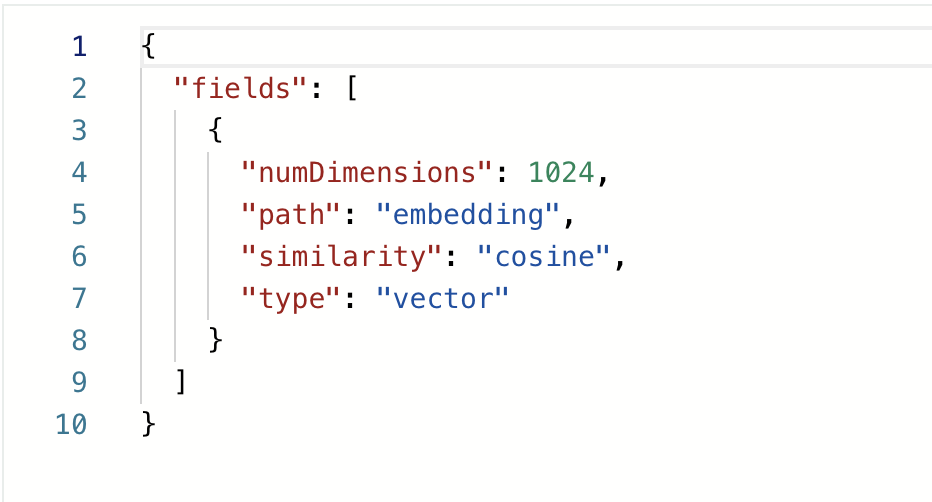
\includegraphics[width=0.8\textwidth]{indexMongoDB.png}
        \caption{Indice vettoriale creato su MongoDB}
        \label{fig:indexMongoDB}
    \end{figure}
    \item \textbf{Generazione della risposta}: le informazioni più pertinenti vengono combinate con la \textit{query} data inizialmente dall'utente per creare un \textit{prompt} che verrà inviato al \gls{llm} che generà la risposta utilizzando il contesto fornito.
\end{itemize}

\subsubsection{\textit{Prompt engineering}}
Come aspetto cruciale per la generazione di proposte di risoluzione di qualità, ho dovuto creare un \textit{prompt} che permettesse al modello di generare proposte di risoluzioni corrette utilizzando il contesto fornito. Inizialmente per testare la qualità del \textit{prompt} creato, ho utilizzato il modello \textit{MistralLarge} di \gls{aws} Bedrock tramite la \textit{console}. La scelta è ricaduta su questo modello in quanto si è dimostrato il più performante tra quelli offerti.
La creazione del \textit{prompt} è stata effettauta ispirandosi alle pratiche del \gls{promptenginnering-g}, ovvero un processo di progettazione e ottimizzazione di \textit{prompt}. L'approccio che ho utilizzato è stato fondamentale un \textit{trial and error} ed è consistito nel testare gli svariati \textit{prompt} creati con il modello \textit{MistralLarge} per valutare la qualità delle proposte di risoluzione generate.
Di seguito mostro il prompt finale creato:
\begin{Verbatim}[frame=single, fontsize=\small]
    Ti fornisco le seguenti informazioni estratte dai documenti:
    ${JSON.stringify(results)}.
    La domanda posta è: "${queryText}".
    
    Istruzioni per la risposta:
    1. Rispondi ESCLUSIVAMENTE in base alle informazioni contenute nei 
       documenti forniti.
    2. NON aggiungere interpretazioni, opinioni o ragionamenti personali.
    3. Se i documenti trattano problemi simili, fornisci TUTTE le possibili 
       soluzioni basate sulle risoluzioni presenti.
    4. Descrivi in modo chiaro ed esaustivo OGNI soluzione possibile, 
       senza limitarti a una sola opzione.
    5. Se le informazioni necessarie non sono presenti nei documenti e i 
       problemi non sono simili, dichiara ESPLICITAMENTE l'impossibilità di 
       rispondere.
    6. La risposta deve essere in lingua italiana.
    7. Inizia SEMPRE la risposta con "In base ai precedenti ticket:".
    8. Includi link nel formato:
       https://${process.env.JIRA_DOMAIN}/jira/servicedesk/projects/
       ${process.env.JIRA_PROJECT_KEY}/queues/custom/66/${key}
    9. Utilizza il seguente formato per ogni soluzione, se disponibile:
        -[Chiave del ticket][Descrizione dettagliata della risoluzione][Link]
    
    10. Se non è possibile fornire una risposta, specificalo 
        chiaramente SENZA aggiungere ulteriori informazioni o speculazioni.
    
    Attieniti RIGOROSAMENTE a queste istruzioni senza deviazioni.
\end{Verbatim}
\subsubsection{Selezione del modello LLM}
La selezione del modello rappresenta una scelta cruciale per una proposta di risoluzione coerente e di qualità. Come ho mostrato nella tabella \ref{tab:prevAttività} ho creato un \textit{benchmark} per selezionare quale tra i modelli più performanti offerti da \gls{aws} Bedrock fosse il migliore per il contesto dei due progetti.
Per la creazione del \textit{benchmark} ho creato una serie di \textit{ticket} fittizzi a cui ho associato delle proposte di risoluzione in base ai \textit{ticket} completati contenuti nel \textit{database}. In seguito, per ognuno di questi ticket veniva richiesta una proposta di risoluzione ai vari modelli da testare e le risposte venivano valutato da un ulteriore modello, di cui ho avuto modo di poterne testare l'accuratezza tramite la \textit{console} di \gls{aws} Bedrock.
\begin{figure}[H]
    \centering
    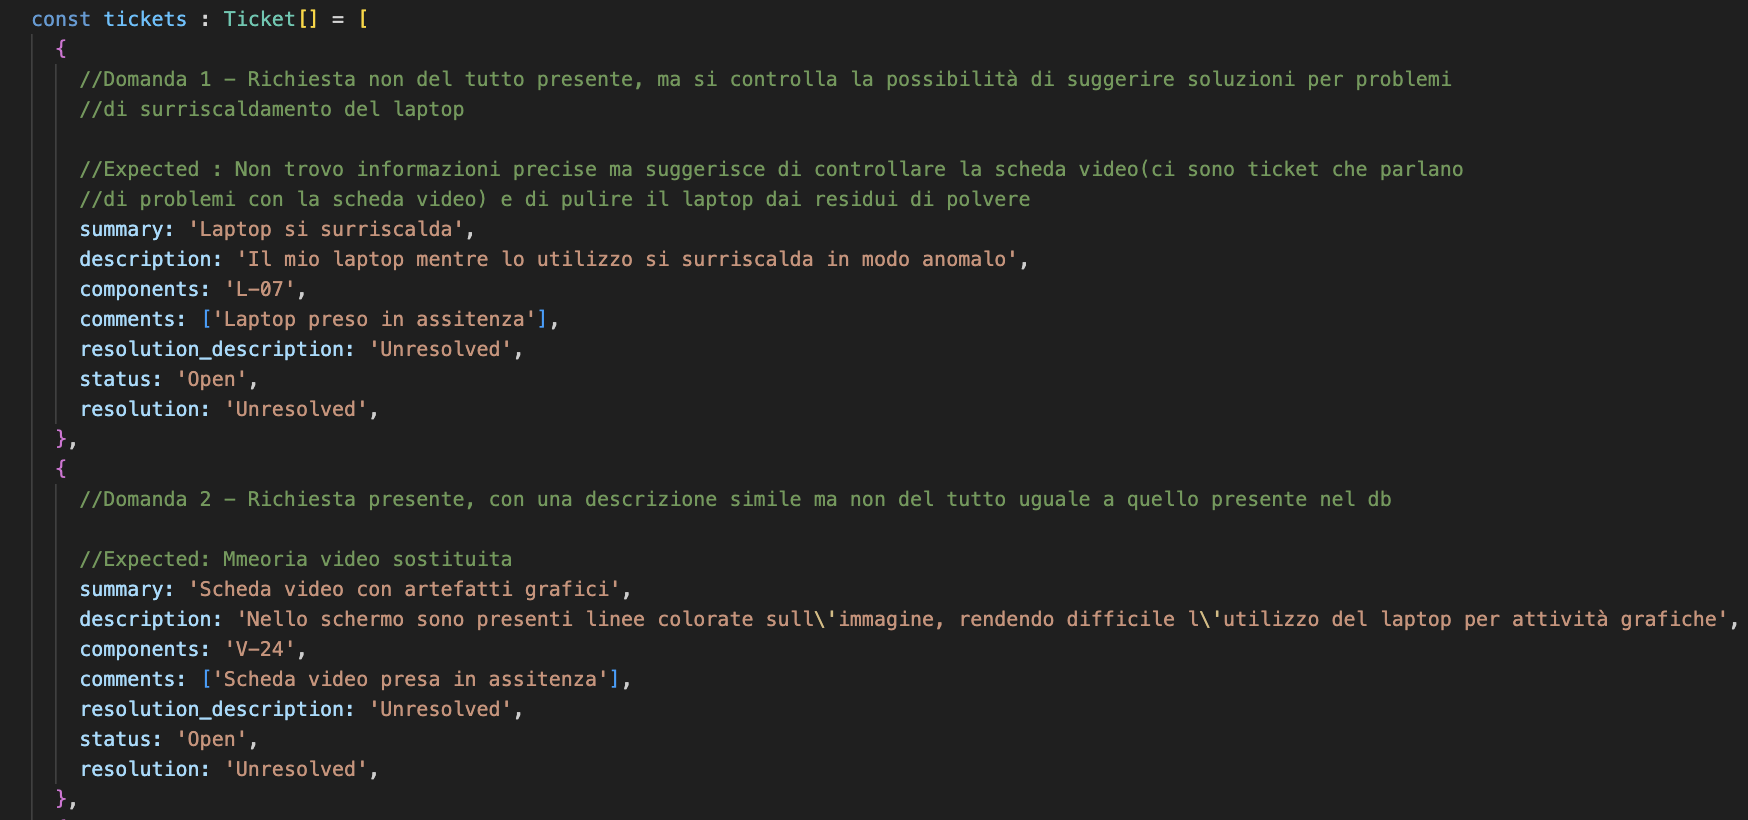
\includegraphics[width=1\textwidth]{ticketBenchmarkExample.png}
    \caption{Esempio \textit{ticket} fittizzi creati per il \textit{benchmark}}
    \label{fig:Ticketbenchmark}
\end{figure}
\noindent
Come mostro nell'immagine \ref{fig:Ticketbenchmark}, i \textit{ticket} creati possiedono tutti i dati che il sistema riceve quando un \textit{ticket} viene creato su Jira. Alcuni di questi dati sono lasciati con valori \textit{default} in quanto lo scopo era quello di valutare la qualità delle proposte di risoluzione dei vari modelli. 
Come sistema di \textit{scoring}, come ho accennato in precedenza, ho utilizzato il modello \textit{MistralLarge} di \gls{aws} Bedrock. Tramite l'utilizzo di questo modello ho potuto attribuire un punteggio di similarità tra la proposta di risoluzione generata dal modello e la proposta di risoluzione attesa in modo automatico. La scala di valutazione del punteggio di similarità varia tra 0 (risposte totalmente diverse) e 1 (risposte identiche). \\
Di seguito mostro l'archittetura del \textit{benchmark}:
\begin{figure}[H]
    \centering
    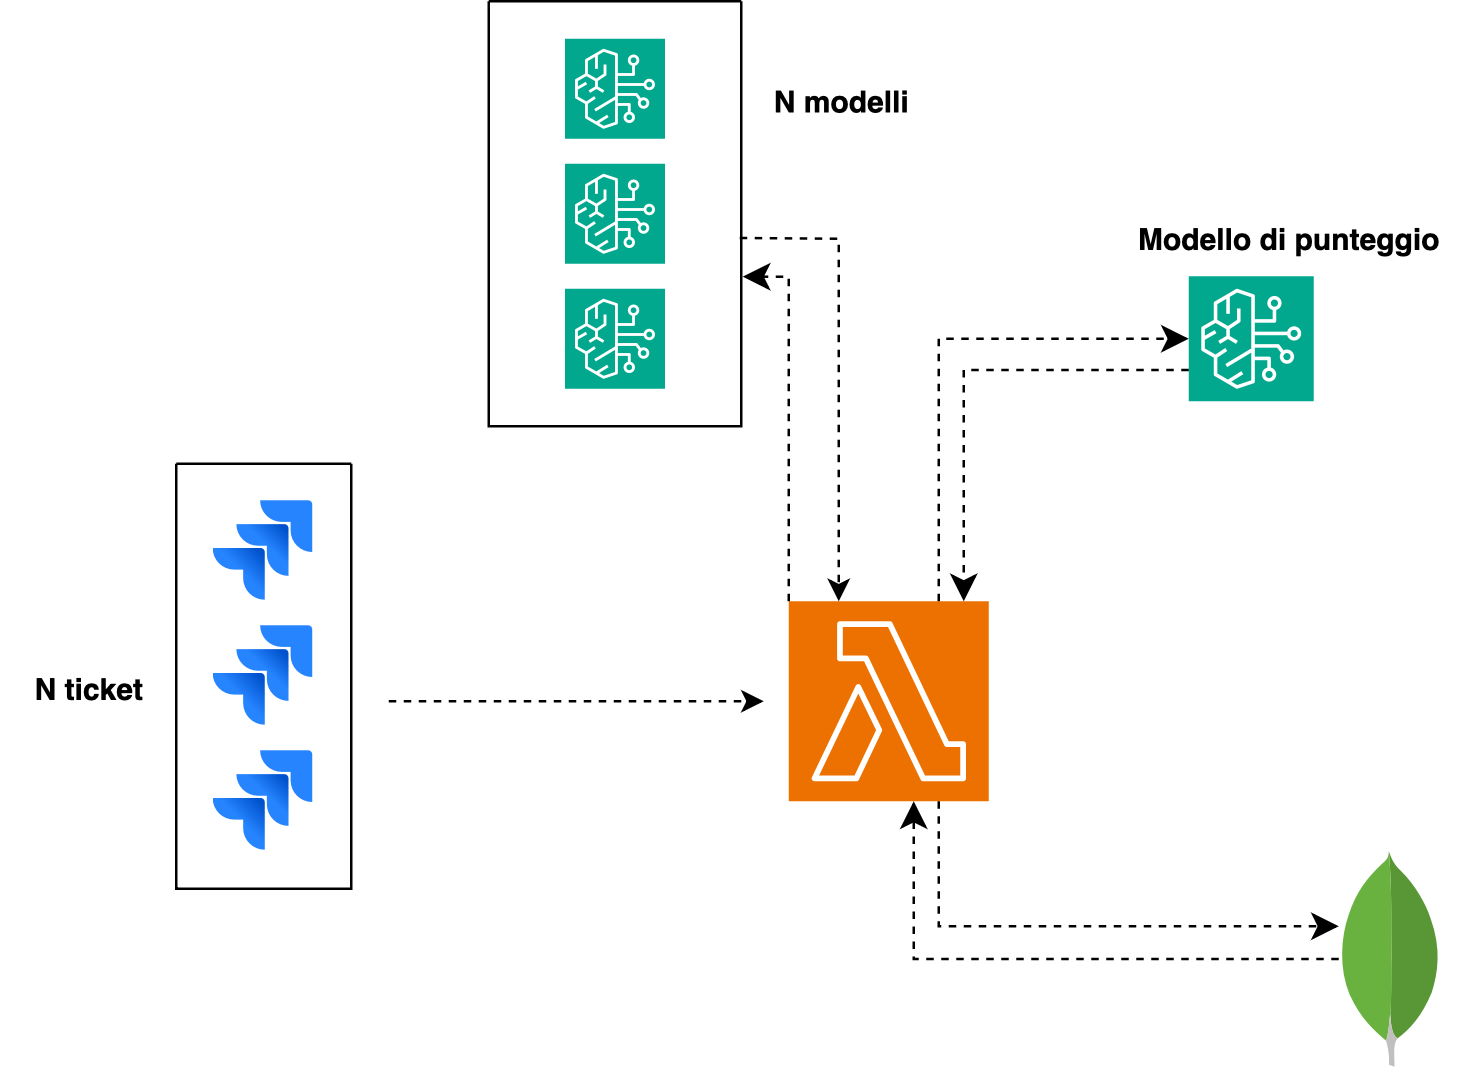
\includegraphics[width=1\textwidth]{architetturaBenchmark.png}
    \caption{Architettura del \textit{benchmark}}
    \label{fig:benchmarkArchitecture}
\noindent
Come mostro nell'immagine \ref{fig:benchmarkArchitecture}, il \textit{benchmark} è composto da tre componenti principali:
\begin{itemize}
    \item \textbf{N \textit{ticket} fittizzi}: insieme di \textit{ticket} creati per valutare la qualità delle proposte di risoluzione dei vari modelli, come mostrato nell'immagine \ref{fig:Ticketbenchmark};
    \item \textbf{N Modelli}: insieme di \gls{llm} offerti da \gls{aws} Bedrock che interrogo per generare proposte di risoluzione per gli N \textit{ticket} fittizzi e li restituisce alla funzione \textit{lambda}; 
    \item \textbf{\textit{Database}}: componente che tramite la ricerca vettoriale trova i \textit{ticket} completati più simili ai \textit{ticket} fittizzi creati. 
    \item \textbf{Modello di punteggio}: modello che valuta la qualità delle proposte di risoluzione generate dai vari modelli interrogati. Restituisce un numero intero positivo compreso tra 0 (risposta totalmente diversa) e 1 (risposta identica).
\end{itemize}
\end{figure}
Di seguito mostro il risultato del \textit{benchmark}:
\begin{figure}[H]
    \centering
    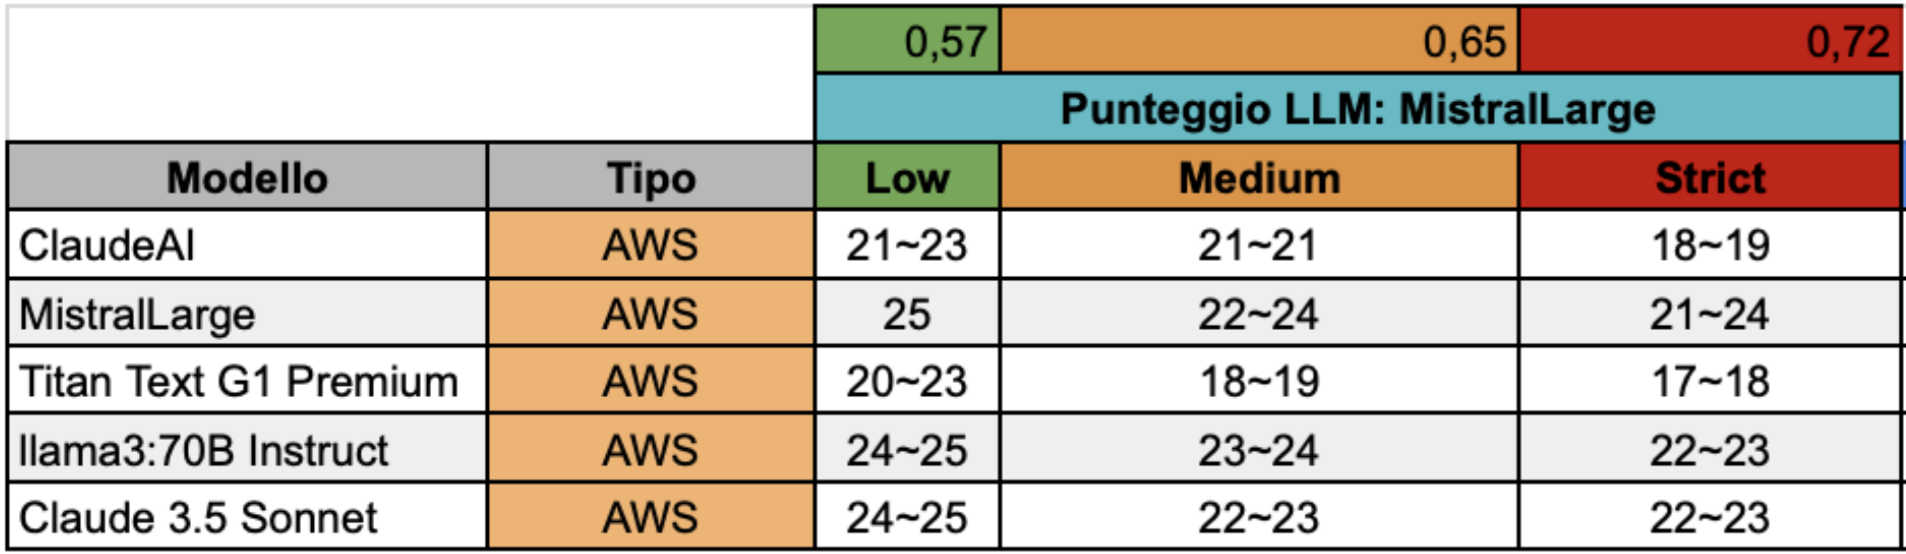
\includegraphics[width=1\textwidth]{benchmark.png}
    \caption{Risultato del \textit{benchmark}}
    \label{fig:benchmarkResult}
\end{figure}
\noindent
Il punteggio relativo ad ogni modello è suddiviso in tre categorie:
\begin{itemize}
    \item \textbf{Low}: punteggio di similarita maggiore di 0,57 incluso;
    \item \textbf{Medium}: punteggio di similarità maggiore di 0,65 incluso;
    \item \textbf{Strict}: punteggio di similarità maggiore di 0,72 incluso;
\end{itemize}
Il punteggio attribuito ai vari modelli però è un indicatore di qualità rispetto alle proposte di risoluzione attese da me create. Questo implica che modelli che hanno ottenuto un punteggio più basso generano comunque proposte di risoluzione corrette, ma non nel formato da me richiesto. Questo è un aspetto che ho dovuto considerare nella scelta del modello.
Come si può notare dall'immagine \ref{fig:benchmarkResult}, il modello \textit{Claude3.5 Sonnet} e \textit{MistralLarge} hanno ottenuto i migliori risultati. Tuttavia la scelta del modello è ricaduta su Claude3.5Sonnet in quanto ha dimostrato di generare proposte di risoluzione di qualità superiore rispetto a \textit{MistralLarge}.\\
Come modello per la generazione di \gls{embedding-g} invece la scelta è ricaduta su \textit{Titan Text Embeddings V2} in quanto rispetto alle alternative offerte da \gls{aws} Bedrock, permetteva di generare \gls{embedding-g} con una dimensione minore ma con una qualità superiore rispetto agli altri modelli.

\subsection{Architettura del sistema \textit{Jira}}
La progettazione delle componenti del sistema Jira si è basata su un'architettura \textit{event-driven}, tipica del \textit{framework Serverless} . Questo tipo di architettura permette di creare applicazioni scalabili e flessibili, in quanto le funzioni \textit{lambda} create vengono eseguite solo quando gli eventi vengono scatenati. 
Durante le prime settimane di \textit{stage} mi è stato fornito un \textit{template} di progetto \textit{Serverless} che ho utilizzato come base per la creazione del sistema Jira. Di seguito elenco le componenti principali del \textit{template} di progetto.

\subsubsection{\textit{Handlers}}
Gli \textit{handlers} sono le funzioni \textit{lambda} che vengono eseguite quando un evento viene scatenato. Esse rappresentano il fulcro del sistema Jira in quanto gestiscono la richiesta di proposte di risoluzione per i nuovi \textit{ticket} e il salvataggio automatico dei \textit{ticket} chiusi in Jira nel \textit{database}. 
Gli \textit{handlers} vengono configurati all'interno del file \textit{serverless.ts} e vengono associati ad un evento specifico. Di seguito mostro un il file di configurazione delle due funzioni \textit{lambda} del sistema Jira

\begin{lstlisting}[caption=Configurazione delle funzioni \textit{lambda} del sistema Jira, label=lst:handlersJira]
    export const tickets: AWS['functions'] = {
      save: {
        handler: `${handlerPath(__dirname)}/handlers/save.main`,
        name: '${self:provider.stage}-${self:service}-save',
        events: [
          {
            http: {
              method: 'any',
              path: 'save',
              cors: true,
            },
          },
        ],
        timeout: 60,
        memorySize: 128,
      },
      suggest: {
        handler: `${handlerPath(__dirname)}/handlers/suggest.main`,
        name: '${self:provider.stage}-${self:service}-suggest',
        events: [
          {
            http: {
              method: 'any',
              path: 'suggest',
              cors: true,
            },
          },
        ],
        timeout: 300,
        memorySize: 128,
      },
    };
\end{lstlisting}
Come mostro nel frammento di codice \ref{lst:handlersJira}, sono presenti due funzioni \textit{lambda}, una rispettivamente per il salvataggio del \textit{ticket} chiuso (funzione \textit{save}) e una per la richiesta di proposta di risoluzione per il \textit{ticket} appena creato (funzione \textit{suggest}).  Entrambe le funzioni sono configurate per essere eseguite quando un evento \gls{httpg} viene scatenato. Definiscono inoltre il tempo massimo di esecuzione e la quantità di memoria allocata per l'esecuzione.

\subsubsection{\textit{Services}}
La componente \textit{services} rappresenta la logica di business. Sono una serie di funzioni di supporto che vengono utilizzate dalle funzioni \textit{lambda} per eseguire operazioni specifiche. Queste funzioni vengono utilizzate per eseguire operazione ad esempio di connessione al \textit{database} o per l'interfacciamento con altri servizi quali ad esempio \gls{aws} Bedrock. Includono funzioni di \textit{parsing} per la gestione delle risposte. 
Questo approccio è vantaggioso in quanto:
\begin{itemize}
    \item \textbf{Modularità}: facilità la manutenzione e la gestione del codice. Ogni funzione ha un compito specifico e ben definito;
    \item \textbf{Riusabilità}: le funzioni di supporto possono essere riutilizzate in altre funzioni \textit{lambda} che si vuole creare;
    \item \textbf{Pulizia del codice}: il codice delle funzioni \textit{lambda} risulta più pulito e leggibile in quanto le operazioni complesse vengono gestite da funzioni di supporto.
\end{itemize}


\subsection*{\textit{Design patterns} utilizzati}
\subsubsection{\textit{\gls{dtog}}}
Il \gls{dtog} è un \textit{design pattern} che viene utilizzato per trasferire i dati tra il \textit{client} e il \textit{server} e viceversa. Utilizzando questo \textit{design pattern} è possibile selezionare i campi che si vogliono trasferire, alleggerendo così il \textit{payload} della chiamata \gls{api}.
\begin{figure}[H]
    \centering
    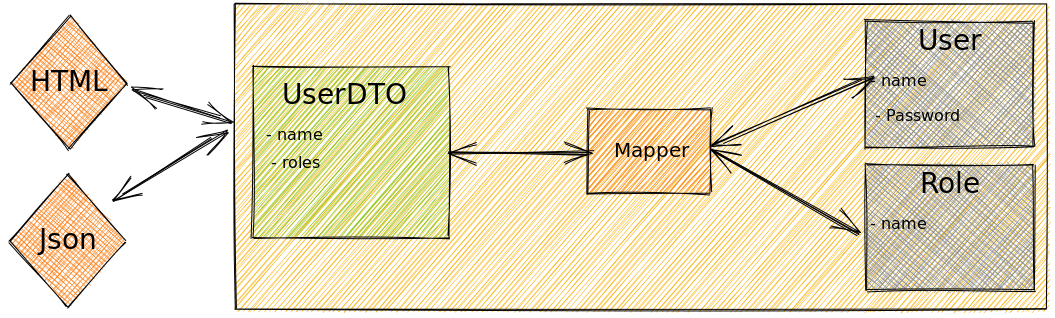
\includegraphics[width=0.9\textwidth]{dto.png}
    \caption{Esempio di utilizzo del \textit{design pattern}}
    \small Fonte: \url{https://www.baeldung.com/java-dto-pattern}
    \label{fig:dto}
\end{figure}

\subsubsection{\textit{Mapper}}
Il \textit{design pattern mapper} è strettamente legato al \gls{dtog}. Come mostro nell'immagine \ref{fig:dto}, il \textit{mapper} consiste in uno o più metodi per facilitare la trasformazione dei \gls{dtog} in oggetti utilizzati dalla logica di \textit{business}, mappando i diversi campi da un tipo all’altro. 
All'interno del sistema Jira, il \textit{mapper} è stato utilizzato per trasformare i dati ricevuti dalle \gls{apig} di Jira in oggetti \textit{ticket} che vengono utilizzati dalle funzioni \textit{lambda} per eseguire le operazioni di salvataggio e di richiesta di proposta di risoluzione.

\subsubsection{\textit{Factory Method pattern}}
Il \textit{Factory Method pattern} è un \textit{design pattern} creazionale che fornisce un'interfaccia per creare un oggetto in una superclasse, ma permette alle proprie sottoclassi di decidere quale classe concreta istanziare. Questo \textit{design pattern} permette di spostare la responsabilità della creazione degli oggetti alla sottoclasse che utilizza il metodo \textit{factory}.
Nel contesto del progetto, il \textit{Factory Method pattern} l'ho utilizzato per la creazione delle interfaccie di connessione con i \gls{llm-g} offerti da \gls{aws} Bedrock. Questo permette in futuro di poter aggiungere nuovi modelli, semplicemente creando una nuova interfaccia di connessione.


\subsection{Architettura del \textit{Chatbot}}
Descrizione dell'architettura del Chatbot tramite il framework Streamlit.
\section{Codifica}
Descrizione dell'attività di codifica delle componenti \textit{AWS Lambda} e del \textit{chatbot}
\section{Verifica e validazione}
Descrizione del processo di Verifica e validazione delle funzione lambda create, attraverso la creazione di eventi di test.
Per quanto riguarda il chatbot, verrà illustrato il perchè non saranno presenti metriche di test.

\section{Risultato finale}
Descrizione del risultato finale ottenuto, ad alto livello.